\chapter{自动驾驶运行时通信系统详细设计与实现}
本章基于概要设计的基础之上,对自动驾驶运行时通信系统各功能模块进行详细设计与实现,主要内容包括系统线程设计、类设计以及
关键算法的描述。

\section{系统软件架构设计}
在概要设计中为了方便本系统向用户提供高抽象能力的接口对本系统进行了层次划分,同时为了便于开发对模块也进行了划分。
本节从代码开发的角度对本系统软件架构的各层次、各模块关系进行明确定义。
本系统的组件图如图\ref{software_component}所示。
\begin{figure}[H]
    \centering
    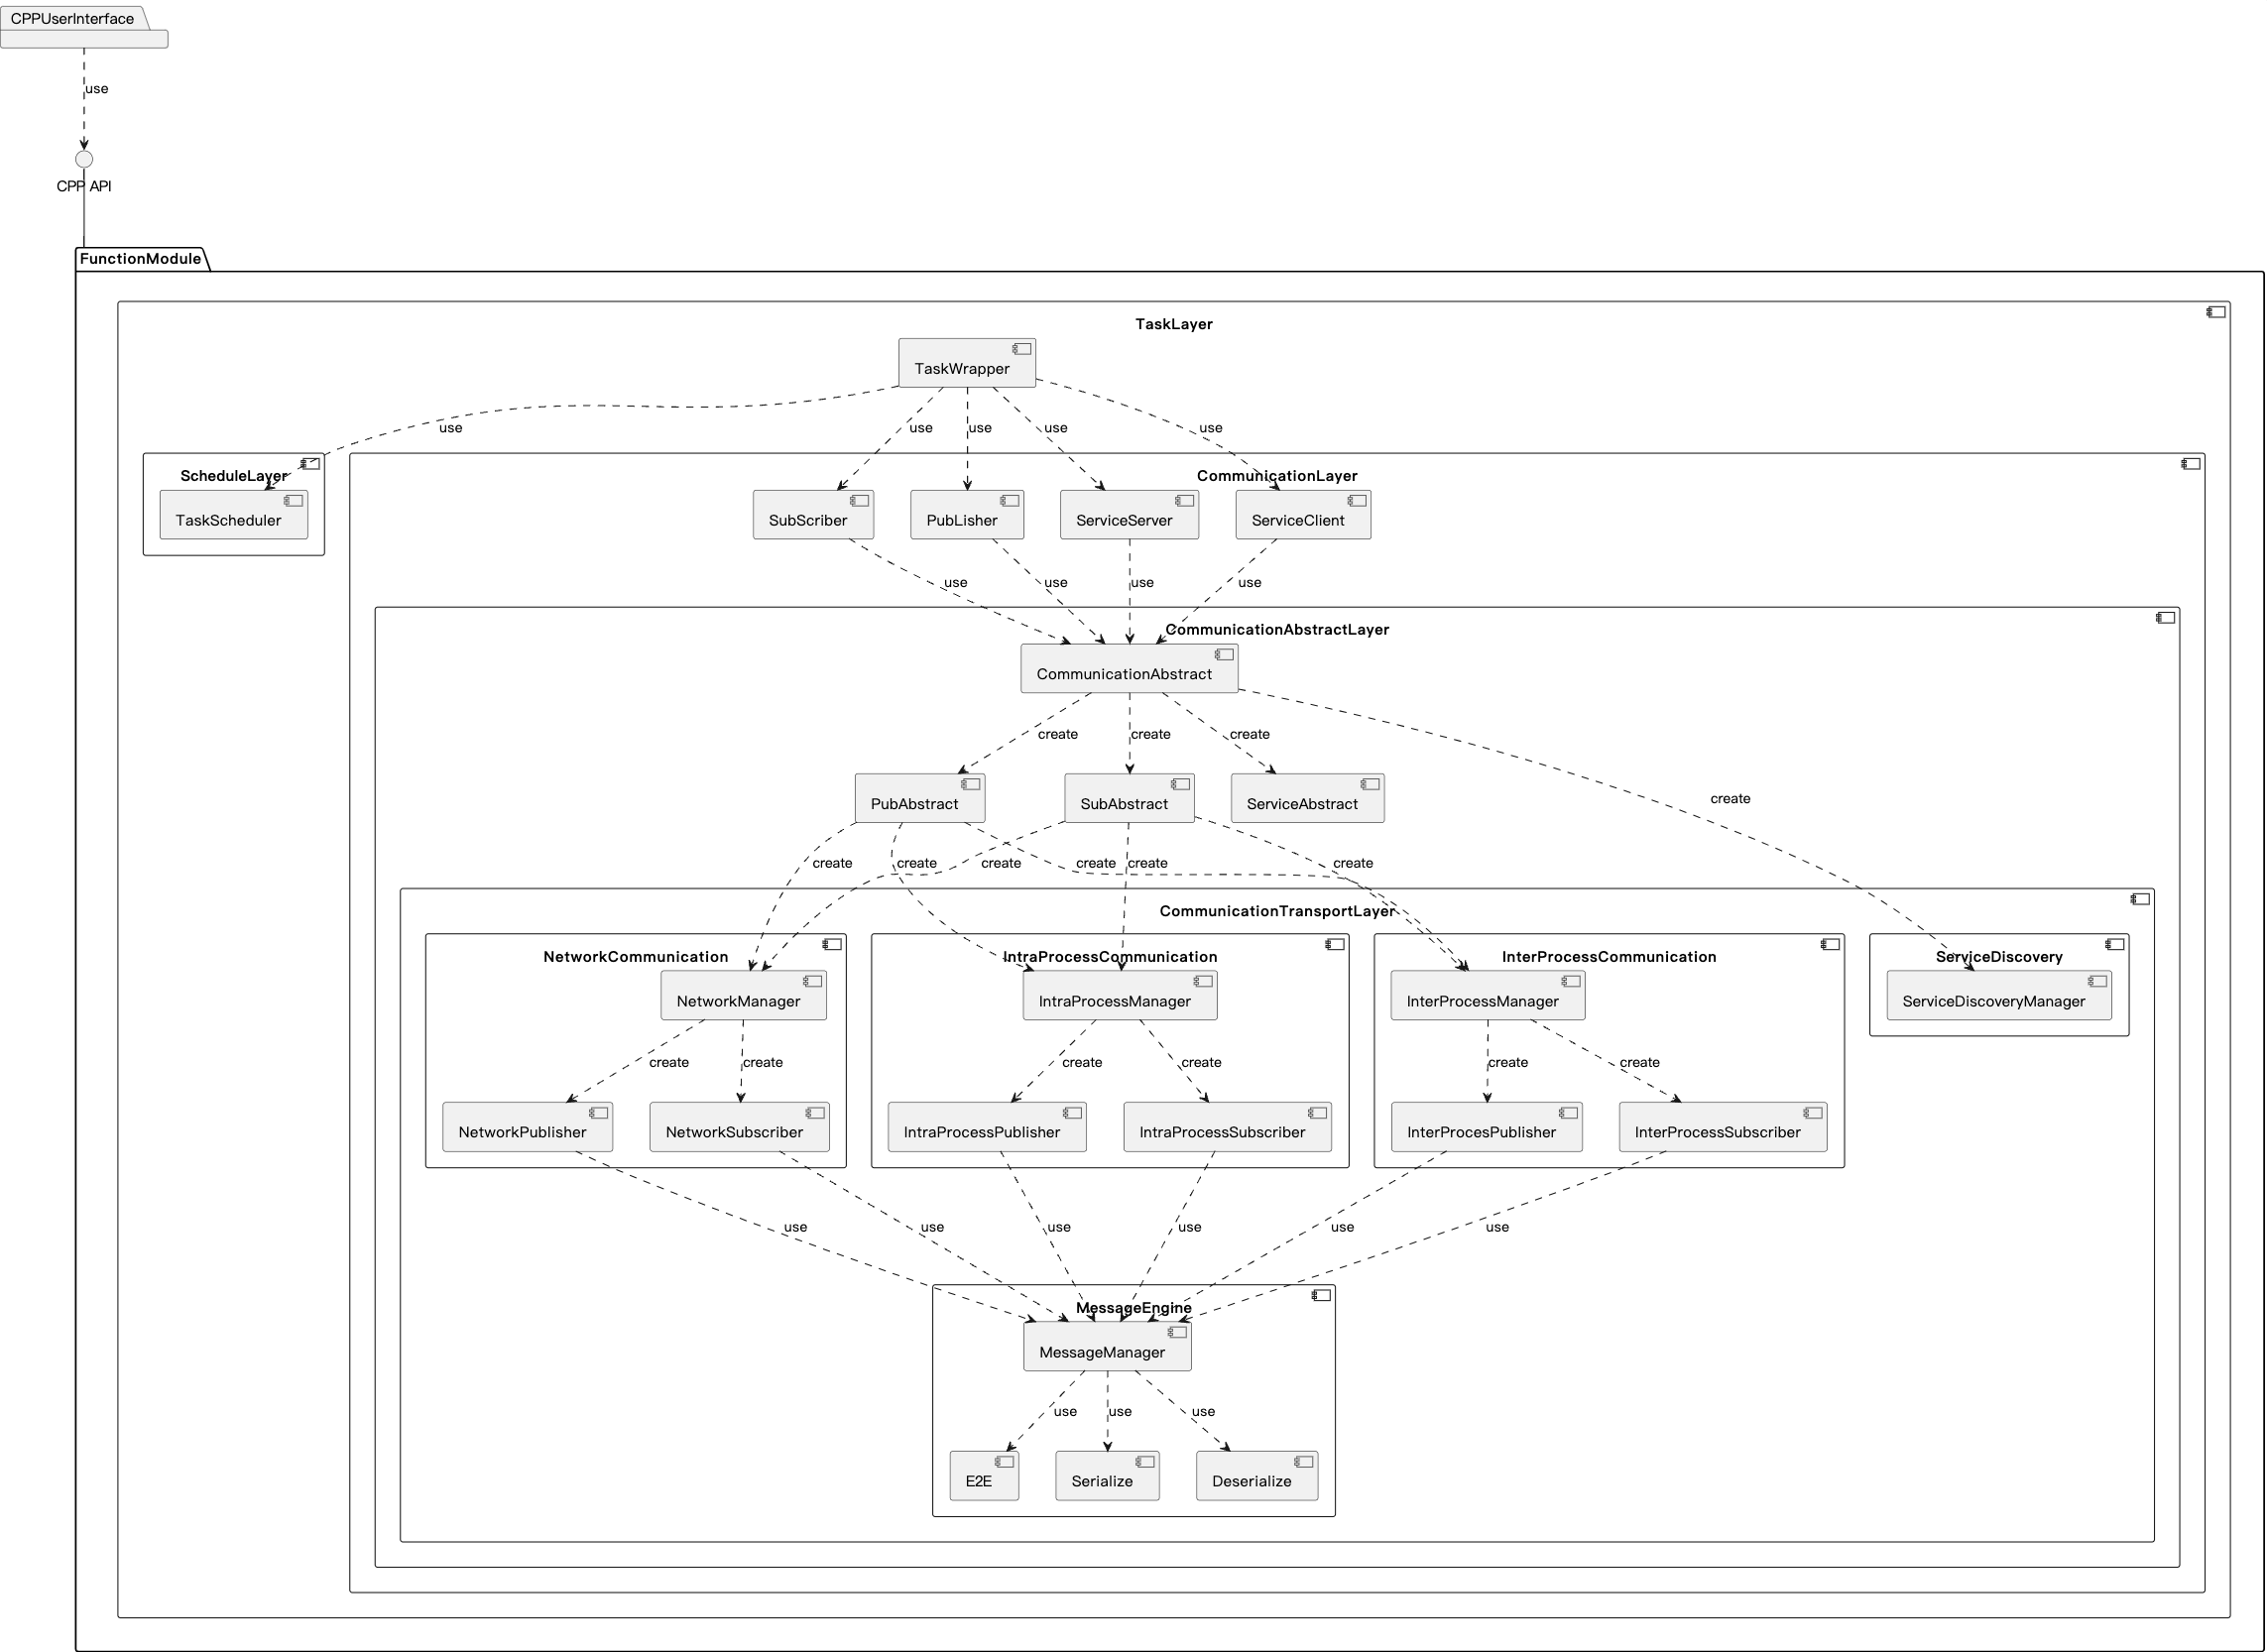
\includegraphics[width=1\textwidth]{software_component.png}
    \caption{自动驾驶运行时通信系统组件图}
    \label{software_component}
  \end{figure}
从图5.1可以看出,本系统在开发阶段严格遵守概要设计阶段对本系统的层次划分以及模块划分规则。

\section{通信单元模块详细设计与实现}
通信单元模块向用户实现了用户管理基于发布-订阅的异步通信的应用程序接口,根据概要设计中提出的设计方案,通信单元模块由发布者模块和订阅者模块
两个二级子模块共同实现功能。发布者模块实现管理发布者以及发布消息的功能,订阅和模块实现管理订阅者以及订阅消息的功能。

\subsection{发布者模块详细设计与实现}
本模块使用C++语言开发并融合其面向对象的编程思想,向用户提供高度抽象的应用程序接口。根据概要设计中的接口设计方案,
发布者模块相关类设计如图\ref{publisher_class}所示。
\begin{figure}[H]
  \centering
  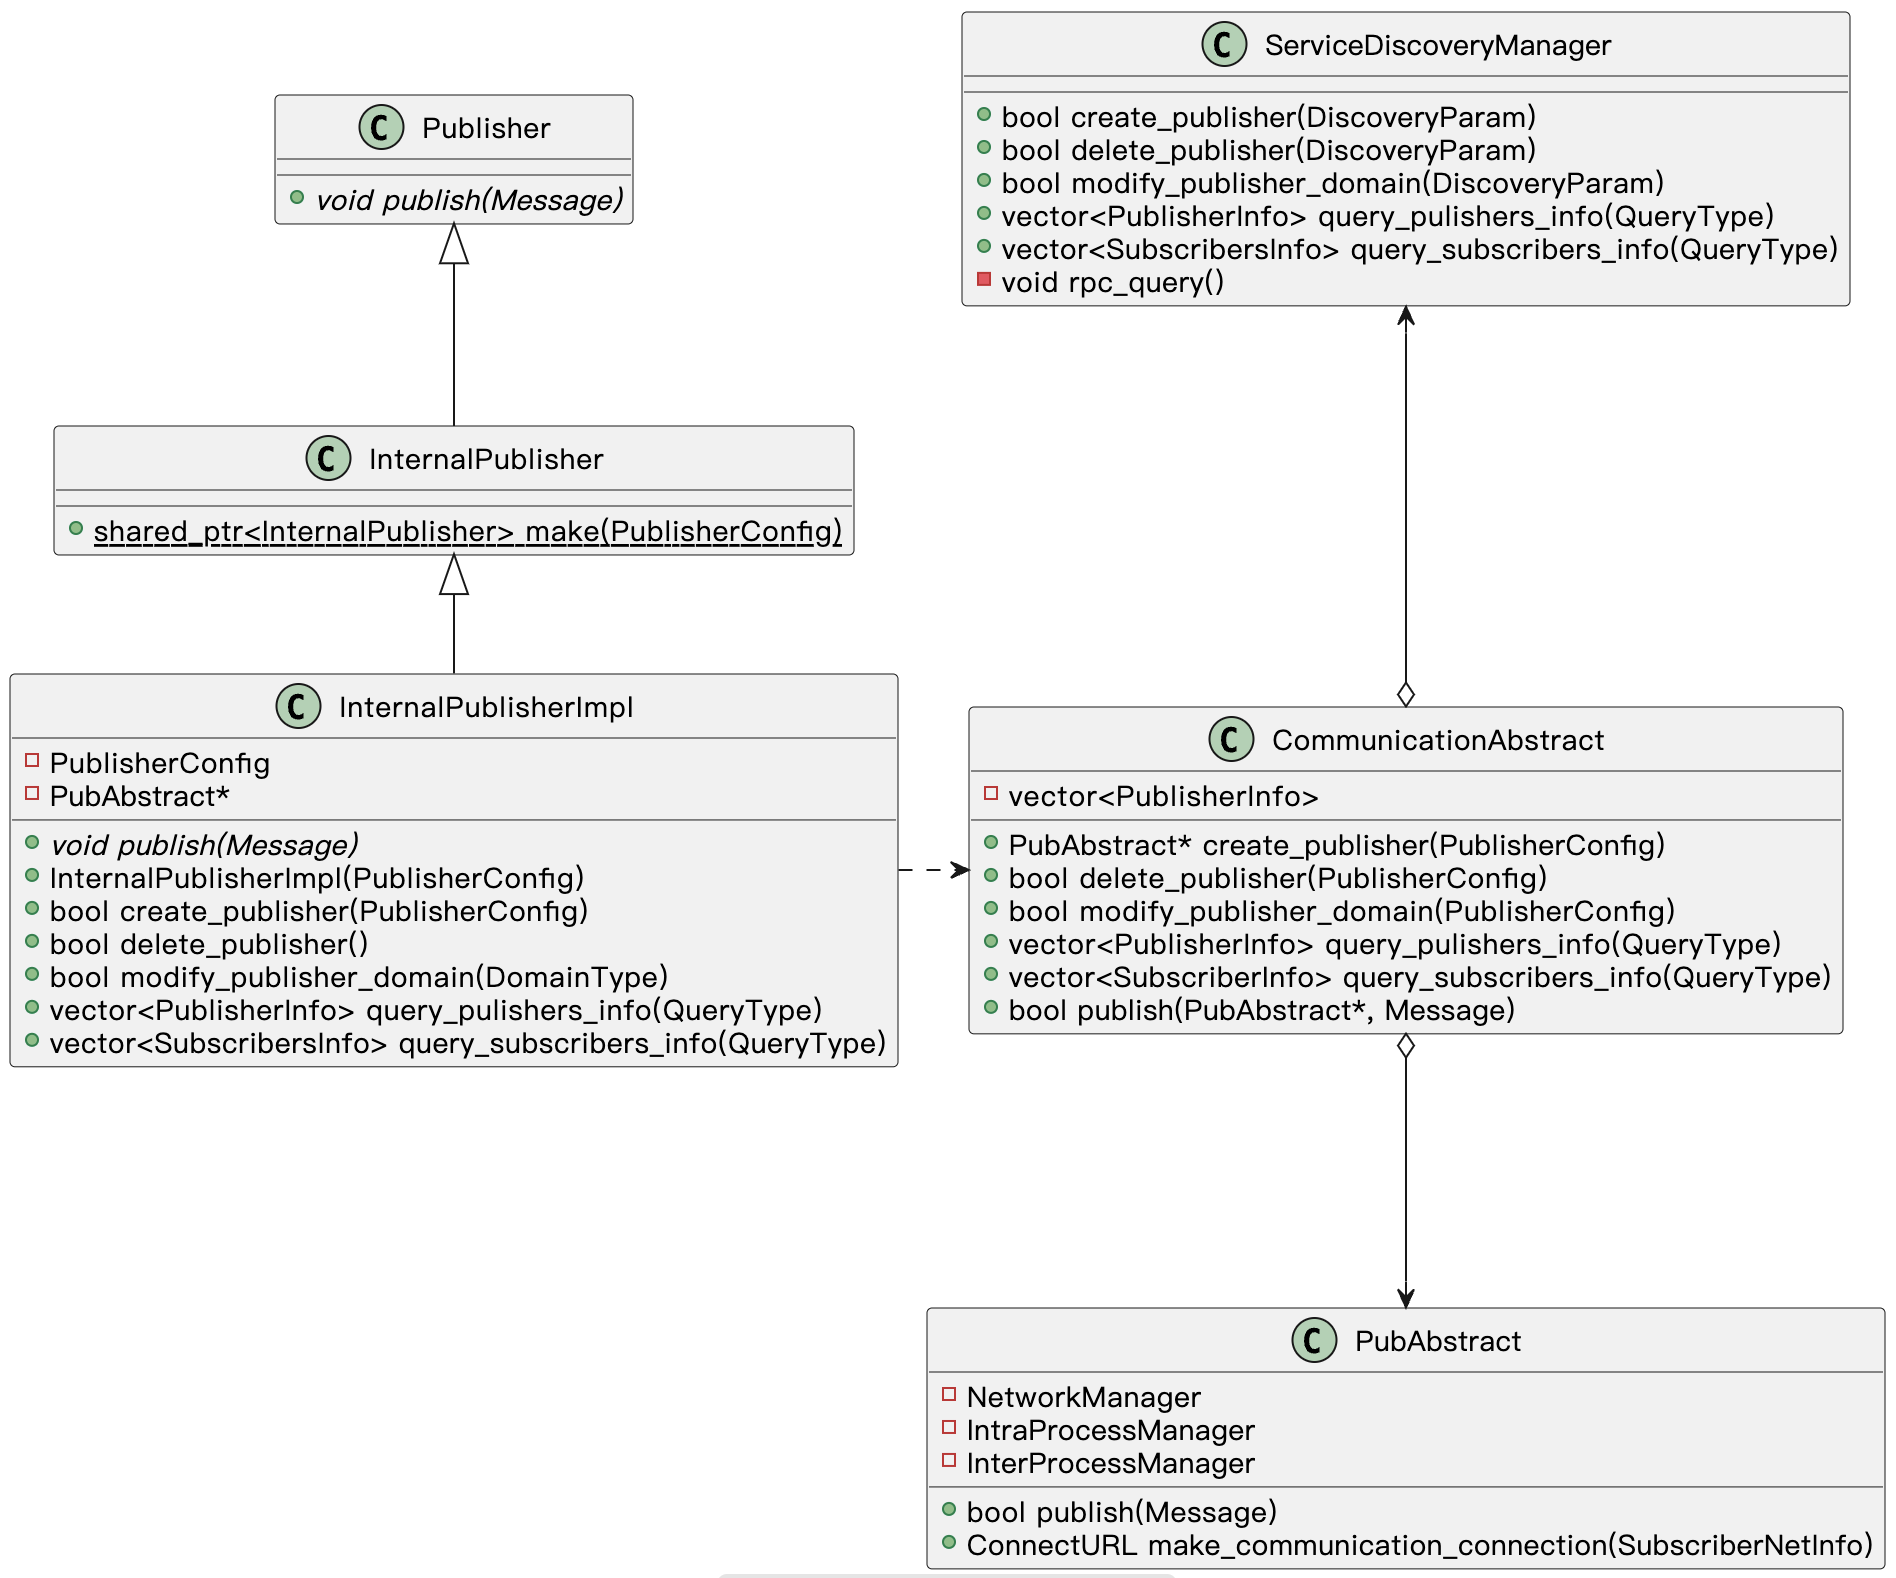
\includegraphics[width=0.9\textwidth]{5.2.png}
  \caption{发布者模块类图}
  \label{publisher_class}
\end{figure}
如图5.2所示,发布者模块主要由Publisher、InternalPublisher和InteralPublisher三个类构成。InternalPublisher
类根据用户传入的发布者配置文件PublisherConfig使用工厂函数make()创建InternalPublisherImpl类,并
通过C++多态的特性将Publisher类的指针指向InternalPublisherImpl类,用户最终使用Publisher类完成管理、发布消息等操作。
InternalPublisherImpl类中保存发布者配置文件PublisherConfig和抽象发布类PubAbstract的指针。
CommunicationAbstract(通信抽象类)、PubAbstract(抽象发布类)和ServiceDiscoveryManager(服务发现类)三个类共同
服务于Publisher类的创建、修改、修改和发布消息功能。

\begin{figure}[htb]
  \centering
  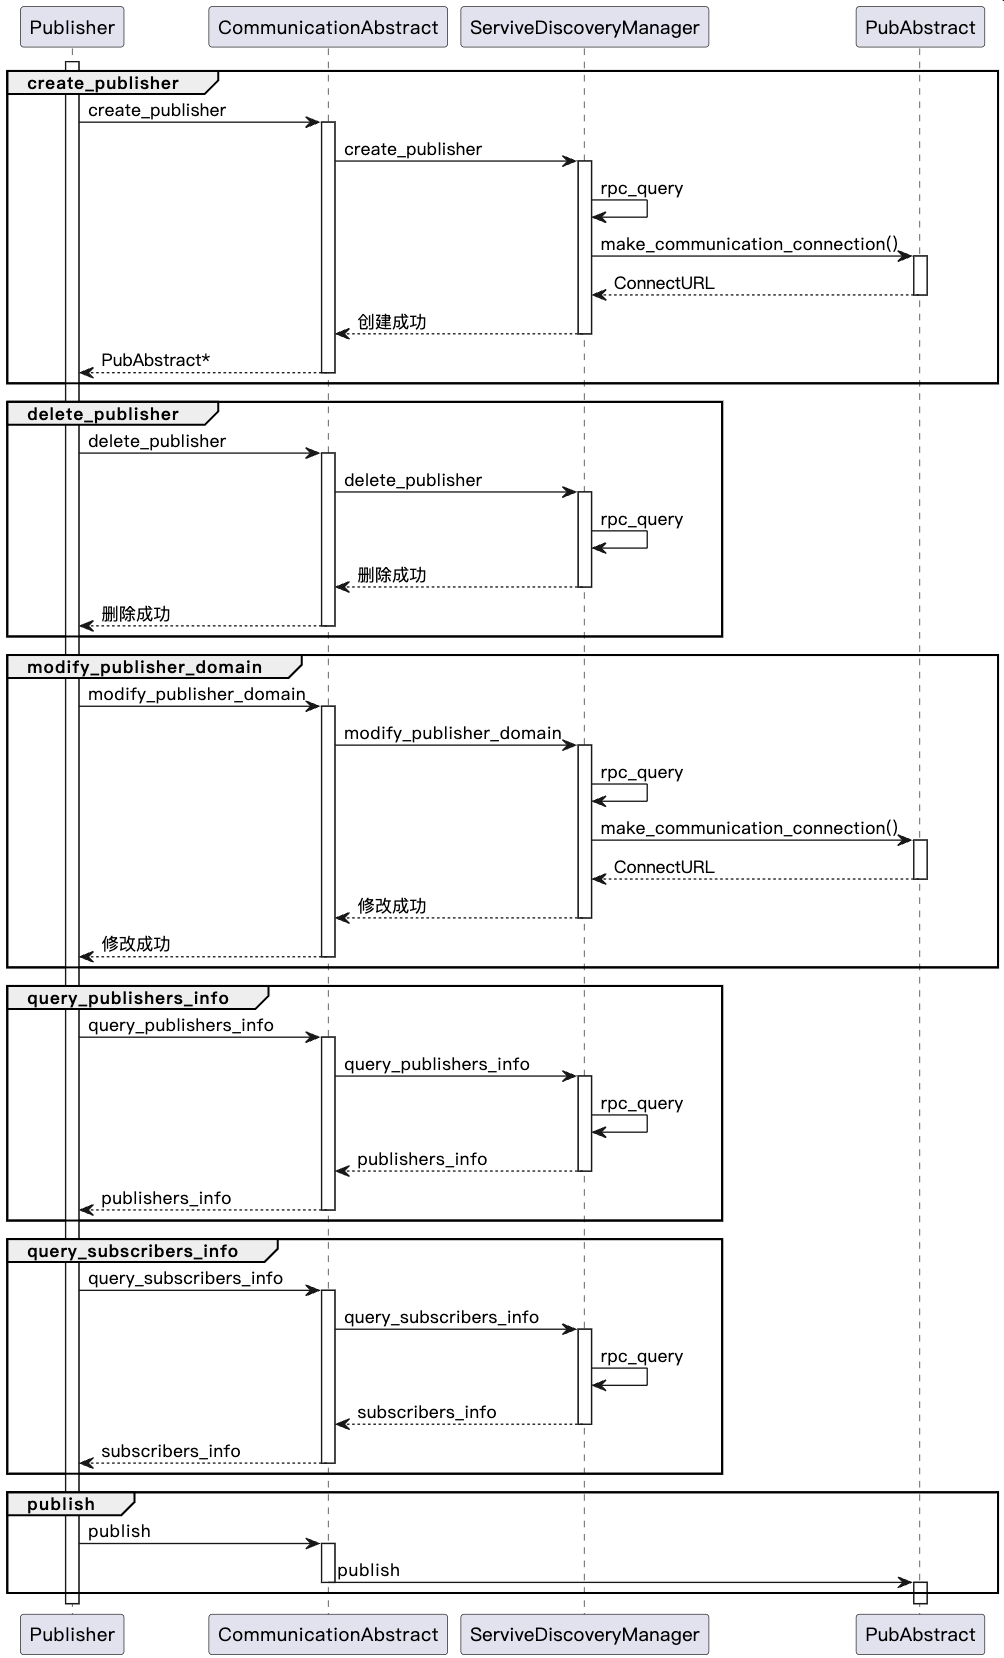
\includegraphics[width=0.81\textwidth]{5.3.png}
  \caption{发布者模块时序图}
  \label{publisher_timesequence}
\end{figure}

发布者模块的时序图如图\ref{publisher_timesequence}所示。
用户创建发布者时,首先调用InternalPublisherImpl类中的create\_publisher函数,函数体内
继续调用CommunicationAbstract类的create\_publisher函数,CommunicationAbstract类创建PubAbstract类
并在PublisherConfig基础上加入IP和进程号生成服务发现参数继续DiscoveryParam调用ServiceDiscoveryManager类中的create\_publisher函数,
ServiceDiscoveryManager类在函数内调用rpc\_query向中心节点发出创建请求完成服务发现工作得到匹配订阅者的网络信息,并调用CommunicationAbstract类绑定的回调函数
在PubAbstract类完成通信链路的建立,最后CommunicationAbstract类返回之前创建的PubAbstract类的指针供
Publisher类调用publish函数发布消息;删除发布者时,调用InternalPublisherImpl类中的delete\_publisher函数,在函数内
继续调用CommunicationAbstract类的delete\_publisher函数,
CommunicationAbstract类首先删除Publisher类对应的PubAbstract类并调用ServiceDiscoveryManager类完成网络拓扑的更新;
修改发布者通信域时,调用InternalPublisherImpl类中的modify\_publisher\_domain函数,在函数内继续调用
CommunicationAbstract类的modify\_publisher\_domain函数,CommunicationAbstract类根据传入的通信域类型
生成服务发现请求参数调用ServiceDiscoveryManager类的modify\_publisher\_domain函数,ServiceDiscoveryManager类
向中心节点发出更改请求完成服务发现工作并调用CommunicationAbstract类绑定的回调函数在PubAbstract类重新建立通信链路。

当用户查询通信系统内的订阅者信息或发布者信息时,首先调用InternalPublisherImpl类中的
query\_publishers\_info或query\_subscribers\_info函数,随后继续调用CommunicationAbstract类
中的query\_publishers\_info或query\_subscribers\_info函数,函数内根据
用户传入的QueryType生成DiscoveryParam调用ServiceDiscoveryManager类中的
query\_publishers\_info或query\_subscribers\_info函数,ServiceDiscoveryManager类根据传入的
QueryType向中心节点查询订阅者或发布者的信息,返回结果。

当用户使用Publisher类中的publish函数发布消息时,publish函数内直接使用InternalPublisherImpl类中保存的
抽象发布类指针PubAbstract*作为参数调用CommunicationAbstract类中的publish函数,CommunicationAbstract类
通过指针调用PubAbstract类中的publish函数,由该类完成对消息的序列化并通过建立的通信链路将消息发布。

\subsection{订阅者模块详细设计与实现}
本模块与发布者模块设计思想一致,向用户提供高度抽象的应用程序接口。根据概要设计中的接口设计方案,
订阅者模块相关类设计如图\ref{subscriber_class}所示。

如图5.4所示,订阅者模块类图设计同发布者模块基本一致,主要由Subscriber、InternalSubscriber和InternalSubscriberImpl
三个类构成。InternalSubscriberImpl内部保存订阅者配置文件和调度配置文件,除了创建、删除和修改通信域三个
函数,该类新增了修改通信方式的函数change\_communication\_mode和一系列操作消息队列的函数。
CommunicationAbstract(通信抽象类)、SubAbstract(抽象订阅类)和ServiceDiscoveryManager(服务发现类)三个类共同
服务于Subscriber类的创建、修改、修改和发布消息功能。不同的是,InternalSubscriberImpl类需要使用Dequeue(双向队列类)
作为消息队列存放订阅到的消息,并使用TaskScheduler(调度类)侵入式地注册基于消息触发的调度策略调度任务。
Dequeue类内部存放了互斥锁保证用户从队列中取出消息和底层通信抽象模块向队列压入消息这两个操作是互斥的,保证数据
的同步性。

\begin{figure}[htb]
  \centering
  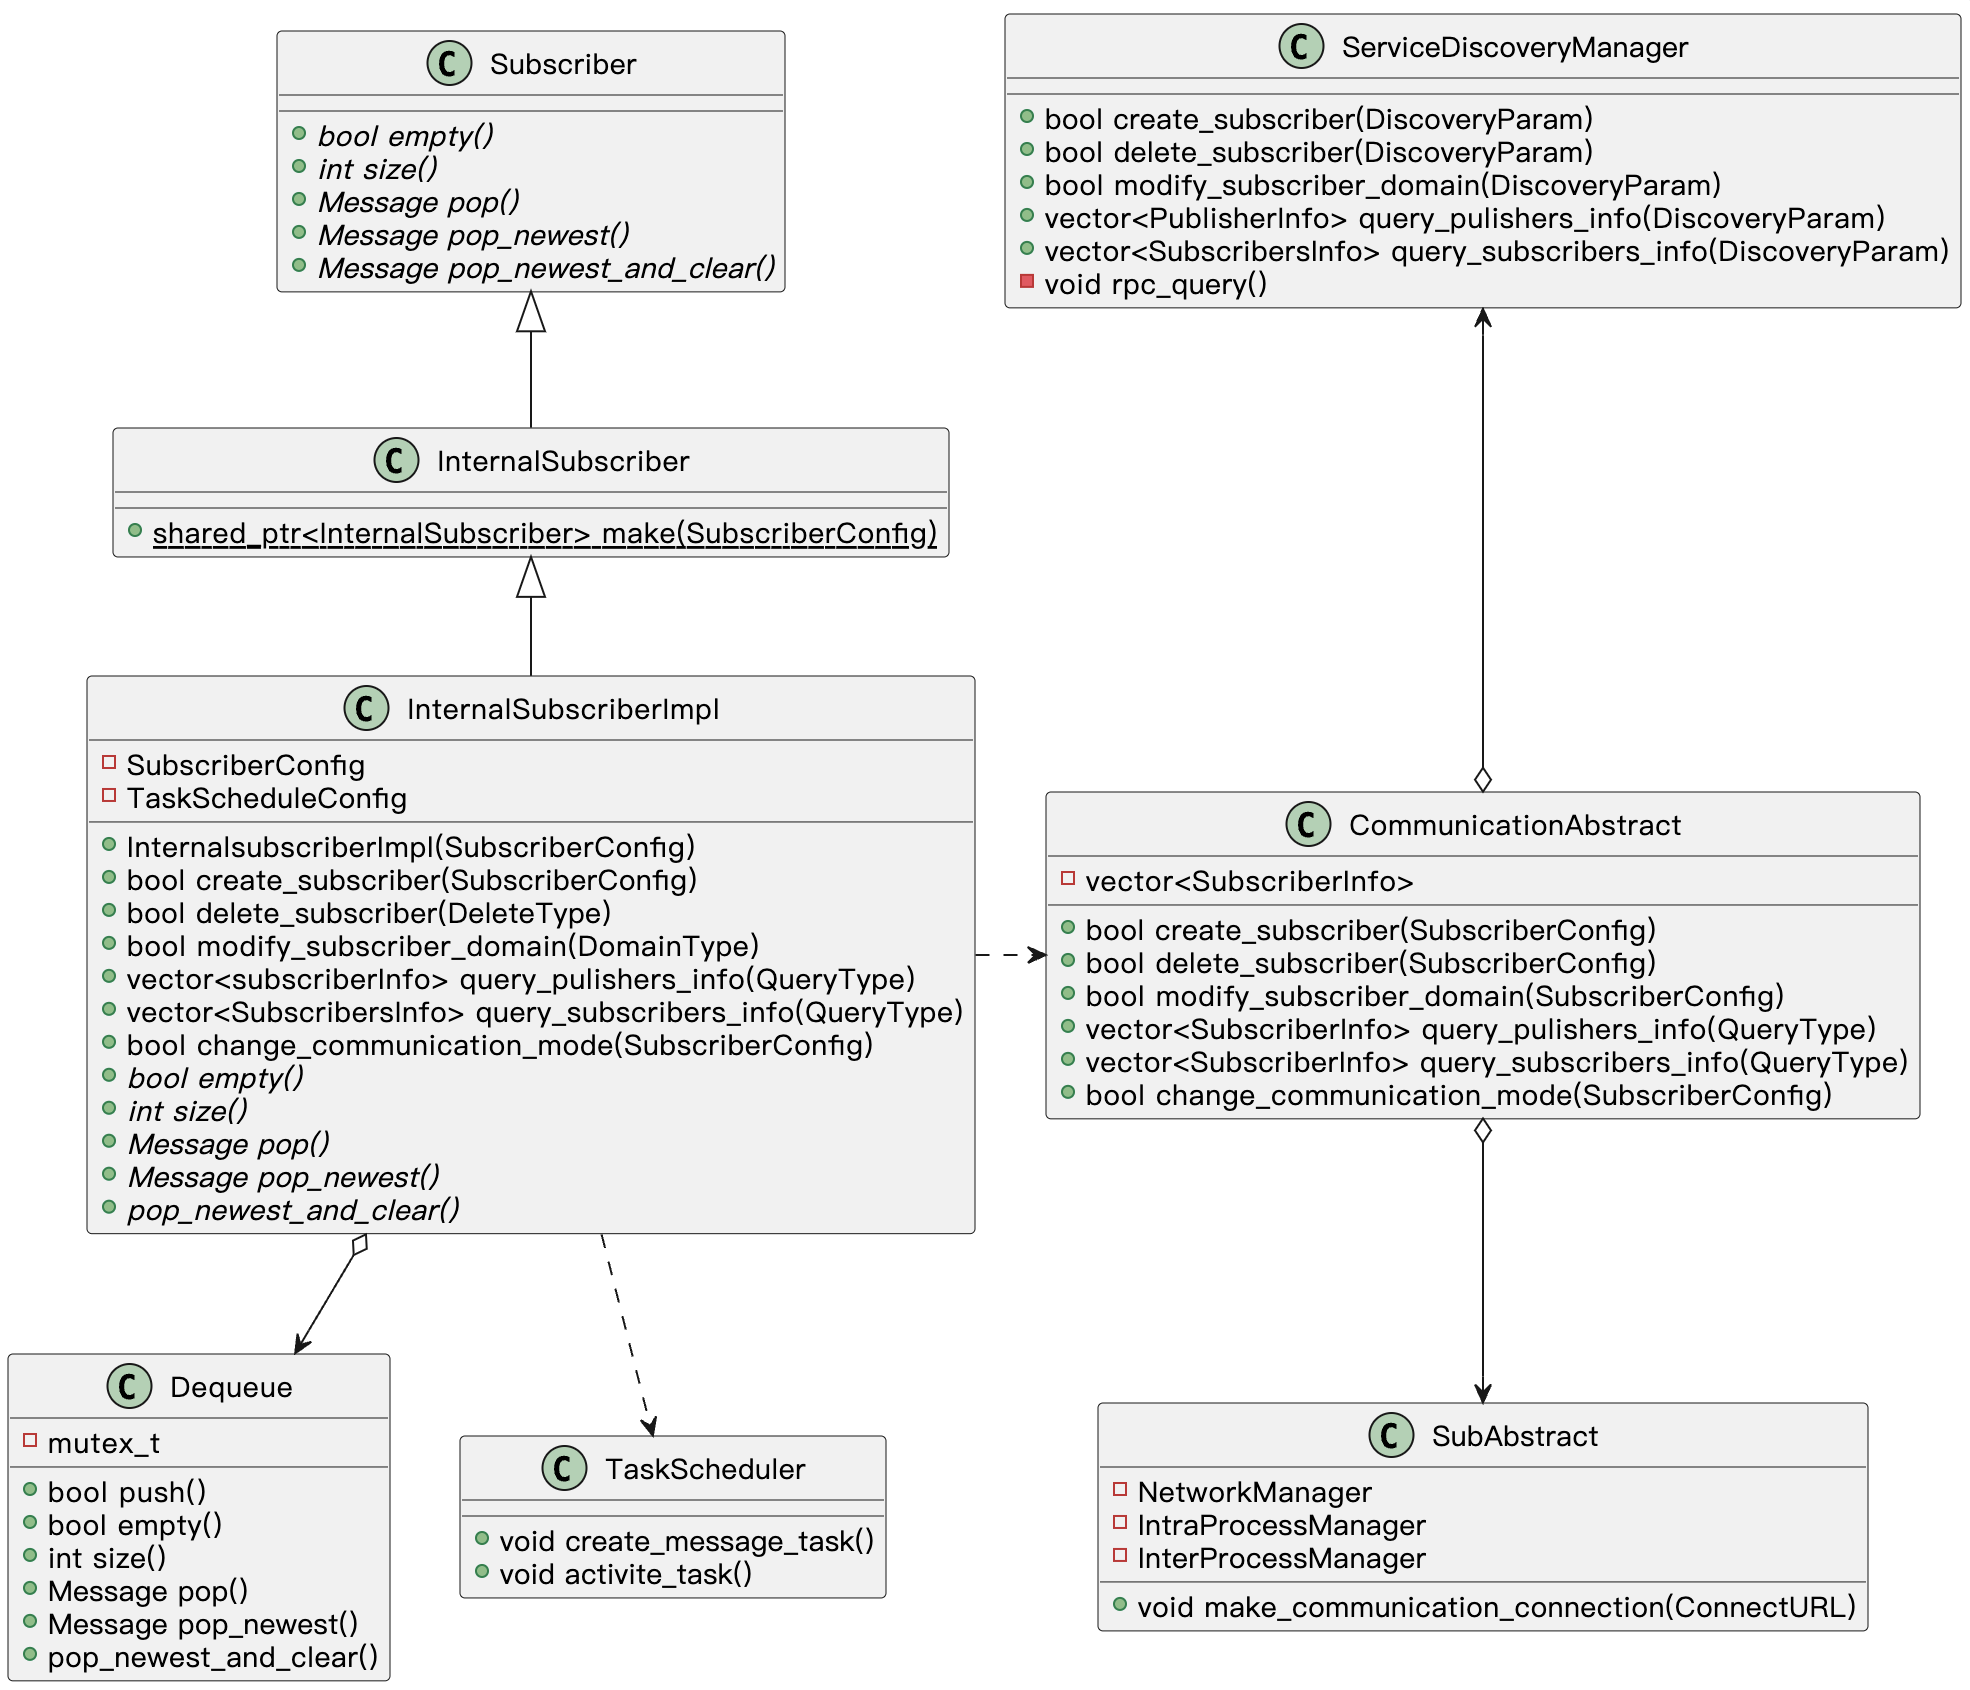
\includegraphics[width=0.85\textwidth]{5.4.png}
  \caption{订阅者模块类图}
  \label{subscriber_class}
\end{figure}

\begin{figure}[htb]
  \centering
  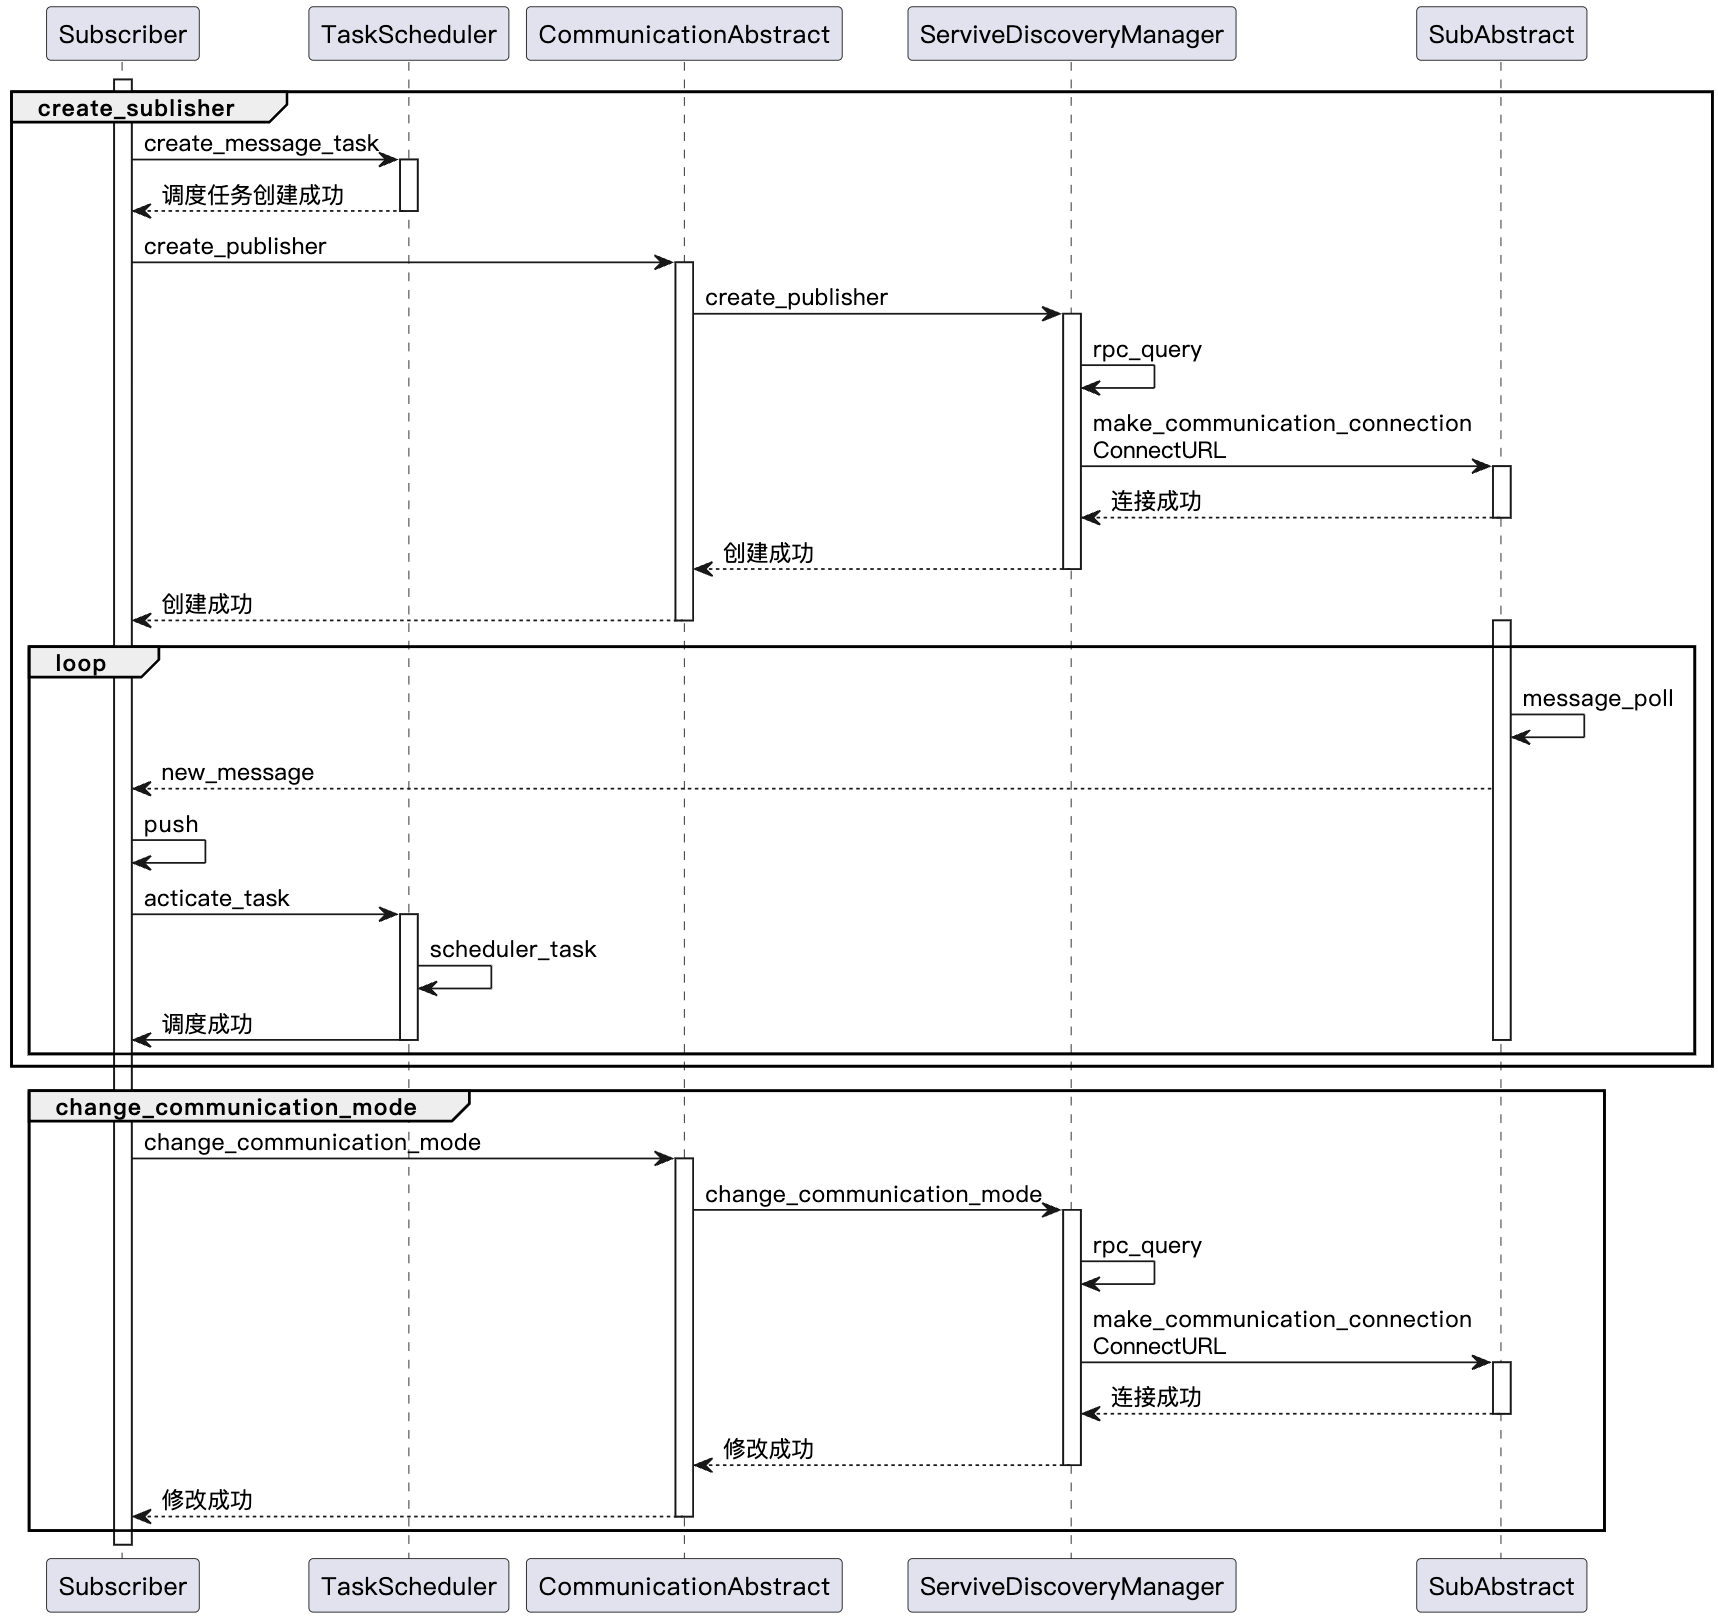
\includegraphics[width=0.85\textwidth]{5.5.png}
  \caption{订阅者模块时序图}
  \label{subscriber_timesequence}
\end{figure}

订阅者模块时序图如图\ref{subscriber_timesequence}所示。
用户创建订阅者时,首先调用InternalSubscriberImpl类的create\_subscriber函数,函数体内设置调度配置文件
ScheduleConfig并调用TaskScheduler类的create\_message\_task()函数创建调度任务并生成相应的回调函数供
SubAbstract类进行回调,回调函数的功能是将新消息压入消息队列并唤醒调度任务,随后继续调用CommunicationAbstract类
的create\_subscriber函数,CommunicationAbstract类在函数中生成服务发现请求参数DiscoveryParam后调用
ServiceDiscoveryManager类的create\_subscriber函数,ServiceDiscoveryManager类调用rpc\_query函数后
得到匹配发布者返回的通信地址后,调用CommunicationAbstract类绑定的回调函数在SubAbstract类中完成通信链路的建立。
SubAbstract类在完成通信链路的建立后开辟轮询新消息的新线程,有新消息到来时调用InternalSubscriberImpl类生成的
回调函数将新消息压入消息队列并唤醒调度任务。

用户修改订阅者通信方式时,首先调用InternalSubscriberImpl类的change\_communication\_mode函数,随后
继续调用CommunicationAbstract类的change\_communication\_mode函数,CommunicationAbstract类
生成服务发现请求参数后调用ServiceDiscoveryManager类的change\_communication\_mode函数,ServiceCommunicationManager
类调用rpc\_query函数后得到匹配发布者返回的通信地址后,最终在SubAbstract类中完成通信链路的建立。

用户删除订阅者时,InternalSubscriberImpl类根据用户传入的删除模式DeleteType判断是否需要将消息队列
中的消息保存至用户空间,随后删除过程同删除发布者过程一致。此外修改订阅者通信域、查询发布者信息和查询订阅者信息这三个操作同发布者模块的过程并无区别,本小节及下一节不再赘述这三种操作的过程。

\section{服务模块详细设计与实现}
服务模块实现了基于RPC请求-应答的同步通信功能,根据概要设计中提出的设计方案,服务模块由客户端和服务端两个二级
子模块共同实现功能。服务端实现管理服务端以及向客户端提供服务的功能,客户端实现管理客户端以及向服务端请求服务的功能。
服务模块设计思想同通信单元模块一致,都采用了面向对象的编程方法,向用户提供高度抽象的应用程序接口。
\subsection{服务端详细设计与实现}
根据概要设计中的接口设计方案,服务端相关类设计如图\ref{server_class}所示。
\begin{figure}[htb]
  \centering
  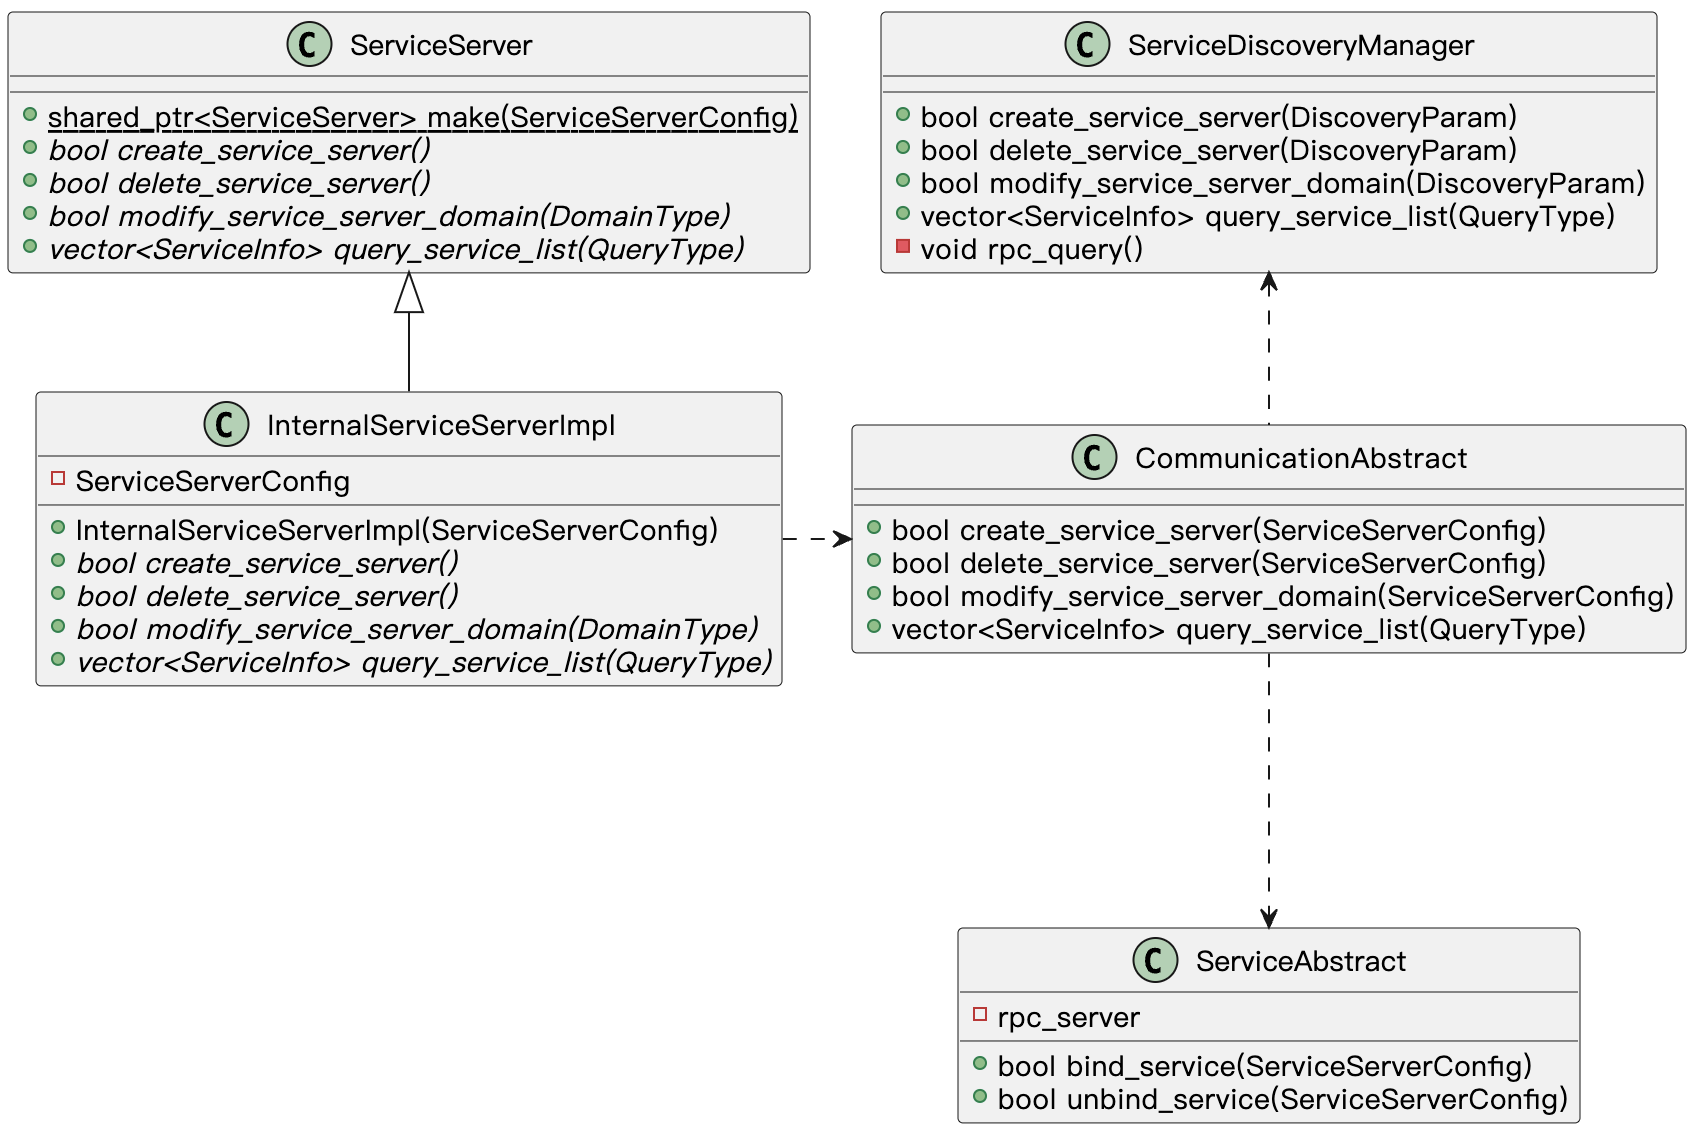
\includegraphics[width=0.85\textwidth]{5.6.png}
  \caption{服务端类图}
  \label{server_class}
\end{figure}

如图5.6所示,ServiceServer类通过make()函数根据传入的服务端配置文件构造实际工作类InternalServiceServerImpl类。
InternalServiceServerImpl类实现了ServiceServer类的所有虚函数,用户基于多态特性通过ServiceServer类即可调用
InternalServiceServerImpl的所有函数。CommunicationAbstract、ServiceDiscoveryManager和SubAbstract三个类
共同完成服务于ServiceServer类的提供服务功能。

服务端时序图如图\ref{server_timesequence}所示。用户通过ServiceServer类中的create\_service\_server函数创建服务端,函数体内继续调用
CommunicationAbstract类中的create\_service\_server函数,CommunicationAbstract类根据用户传入的
服务端配置文件ServiceServerConfig调用ServiceAbstract类中的bind\_service函数,ServiceAbstract类根据
配置文件中的服务名、回调函数绑定服务至rpc服务器,随后CommunicationAbstract类生成服务发现请求参数DiscoveryParam
调用ServiceDiscoveryManager类的create\_service\_server函数,ServiceDiscoveryManager类调用rpc\_query函数
完成向中心节点的注册,返回注册成功。

用户通过ServiceServer类中的delete\_service\_server函数删除服务端,函数体内继续调用CommunicationAbstract类中的
delete\_service\_server函数,CommunicationAbstract类首先调用ServiceDiscoveryManager类在网络拓扑中
删除该服务,随后调用ServiceAbstract类中的unbind\_service函数解除服务的绑定,最后返回删除成功。


\begin{figure}[htb]
  \centering
  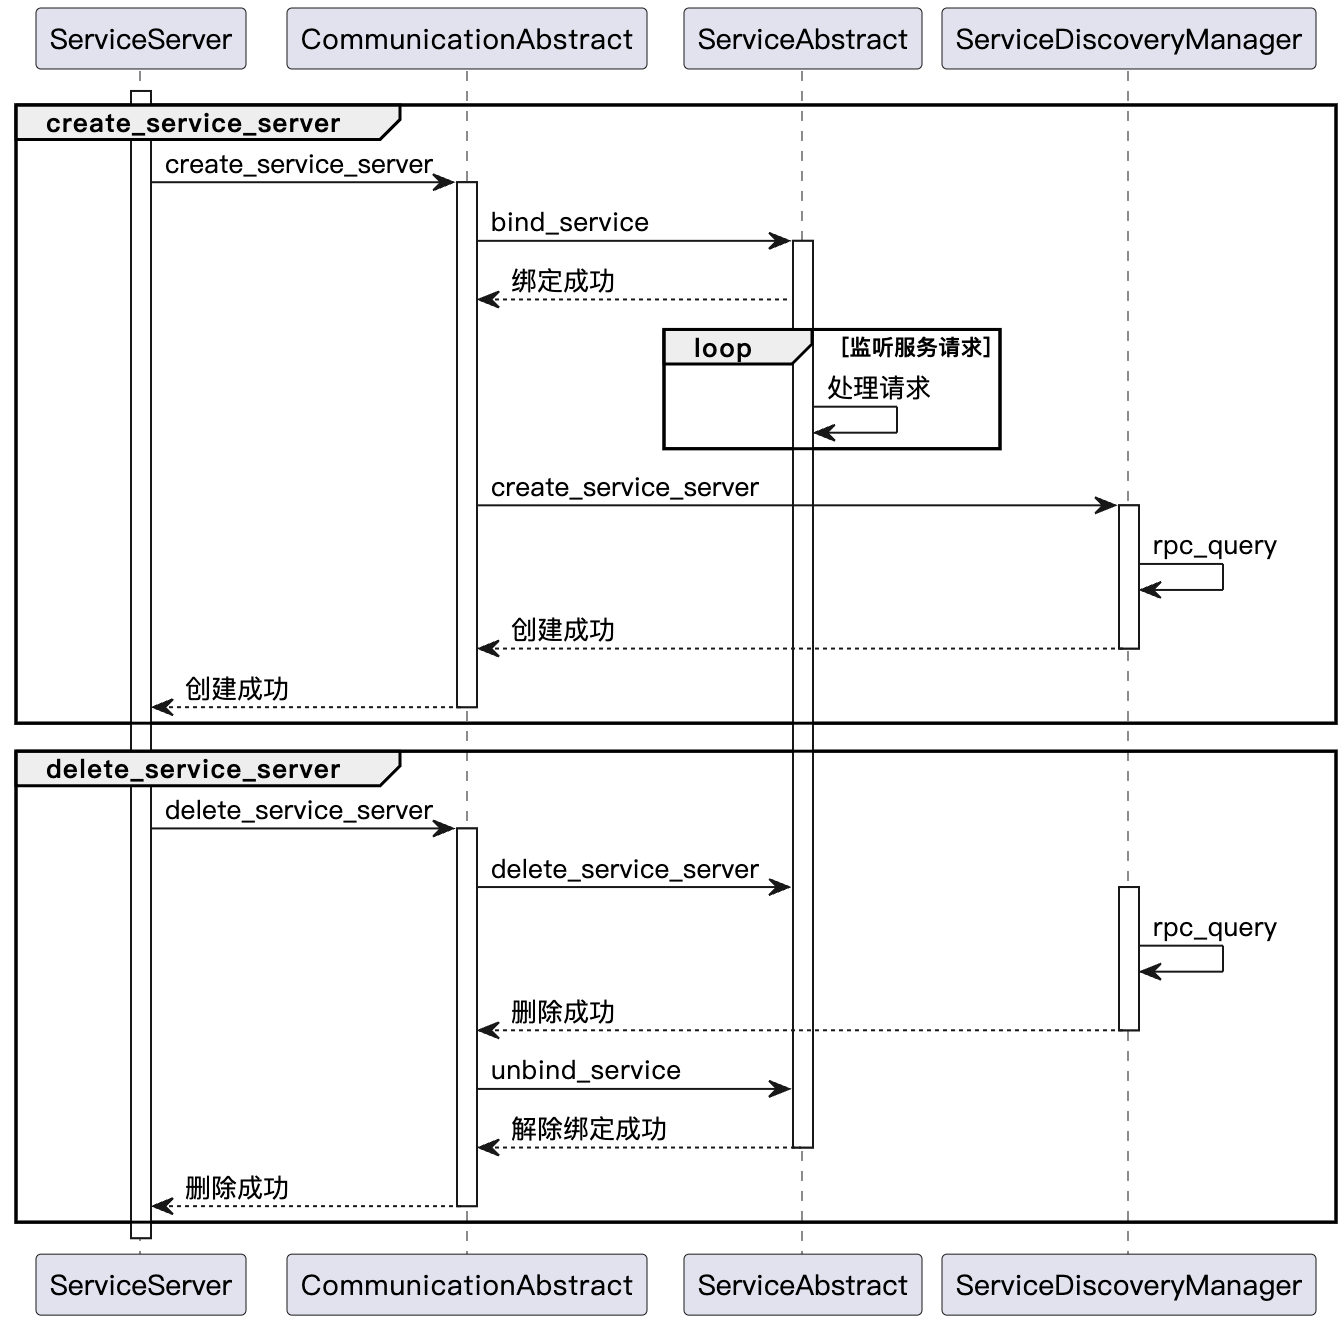
\includegraphics[width=0.85\textwidth]{5.7.png}
  \caption{服务端时序图}
  \label{server_timesequence}
\end{figure}

\subsection{客户端详细设计与实现}
根据概要设计中的接口方案,客户端相关类设计如图\ref{client_class}所示。客户端的设计思想同服务端一致,ServiceClient类通过make()函数根据
传入的客户端配置文件构造实际工作类InternalServiceClientImpl类。InternalServiceClientImpl类实现了ServiceClient类
所有的虚函数。与服务端不同,客户端的注册、删除和修改通信域并不需要ServiceDiscoveryManager类向中心节点发起请求,ServiceDiscoveryManager类
只将客户端配置文件保存至本地。只有在客户端发起实际服务请求时ServiceDiscoveryManager类才向中心节点发起请求。
ServiceAbstract采用单例设计模式,同一个进程中只存在唯一的ServiceAbstract类实例。

\begin{figure}[htb]
  \centering
  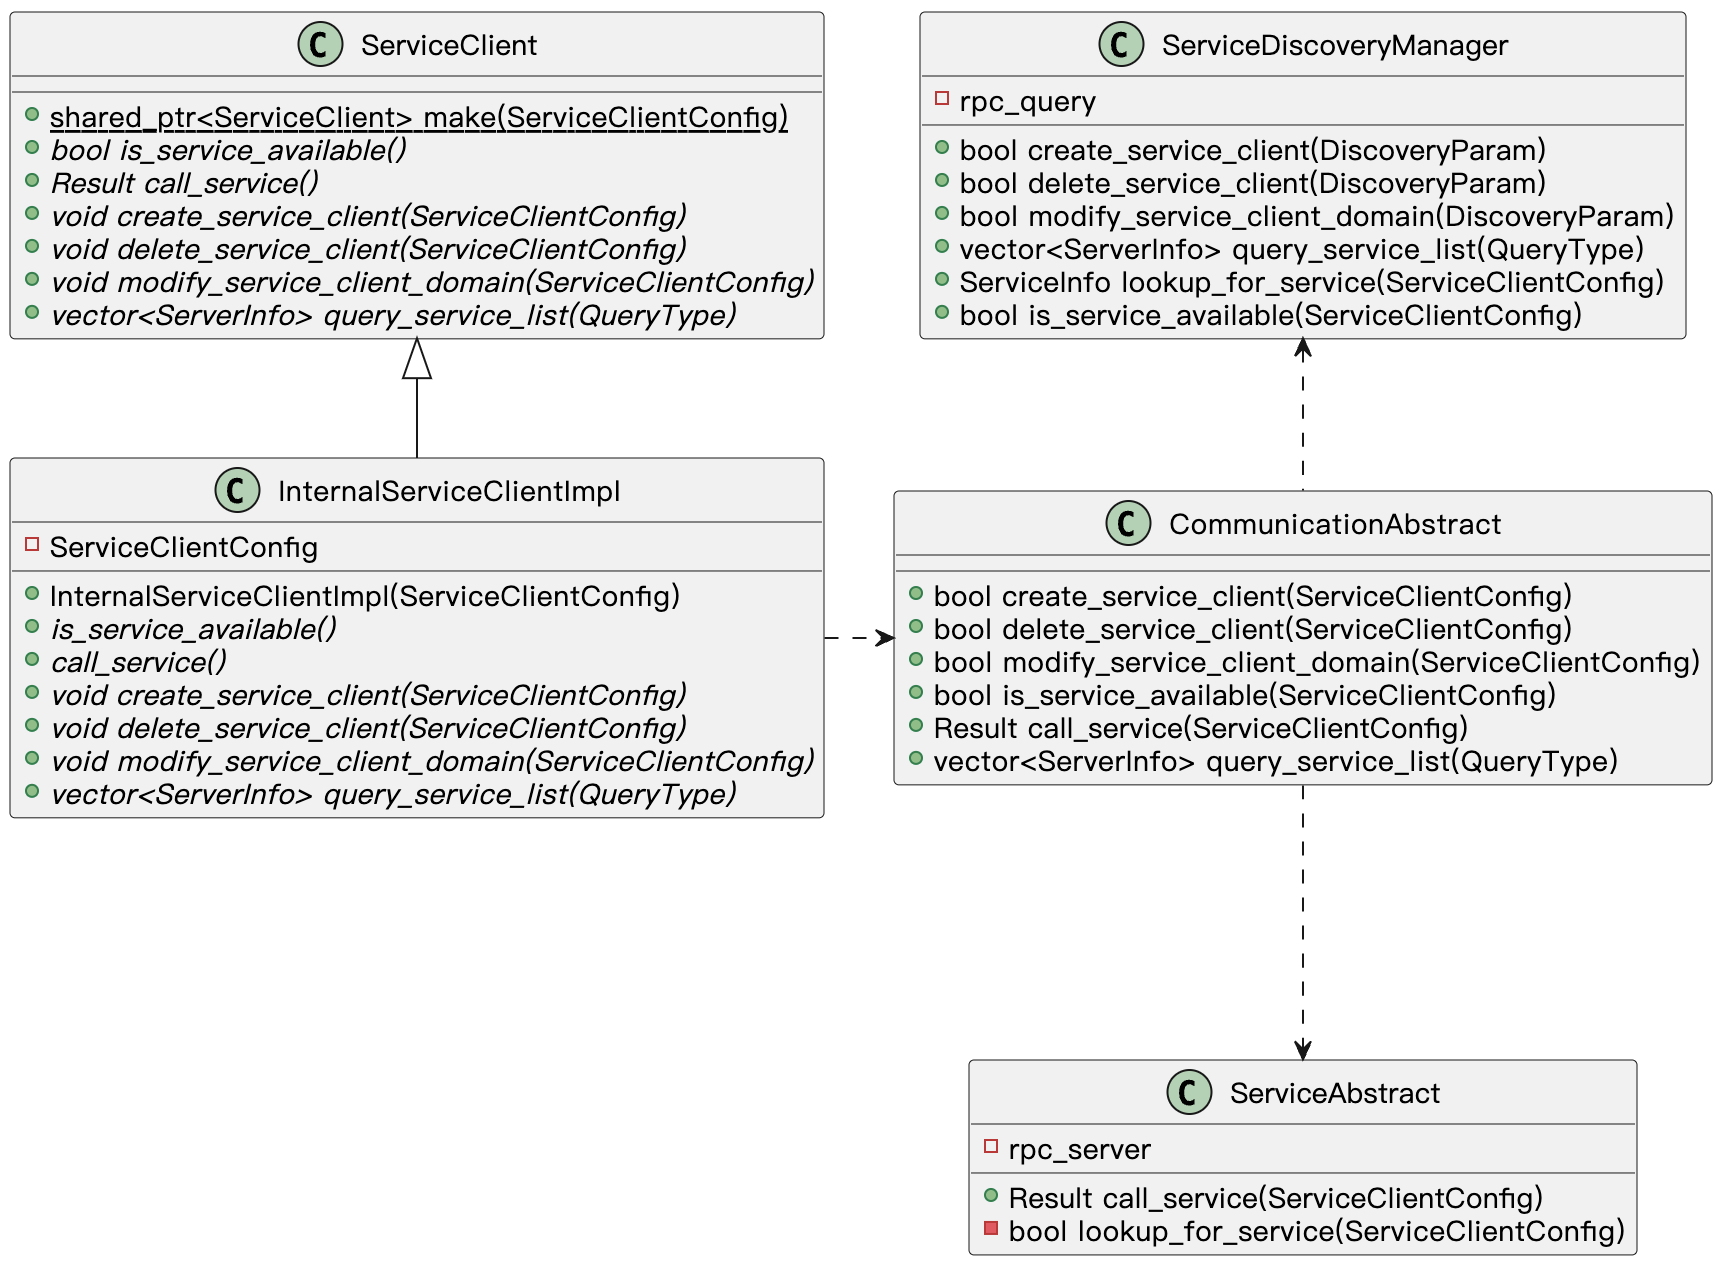
\includegraphics[width=0.85\textwidth]{5.8.png}
  \caption{客户端类图}
  \label{client_class}
\end{figure}
客户端时序图如图\ref{client_timesequence}所示。用户通过ServiceClient类中的create\_service\_client函数创建客户端,函数体内继续调用
CommunicationAbstract类中的create\_service\_client,CommunicationAbstract类将客户端配置文件
ServiceClientConfig保存,随后返回创建成功,创建过程并不需要ServiceDiscoveryManager类参与。此外,用户调用ServiceClient类中的
delete\_service\_client函数和modify\_service\_client\_domain函数同样不需要ServiceDiscoveryManager类参与。

用户通过ServiceClient类中的call\_service函数发出对服务的请求,函数内调用CommunicationAbstract类的call\_service函数
并最终在ServiceAbstract类中call\_service函数执行实际的服务请求。ServiceAbstract类通过调用ServiceDiscoveryManager类中的
lookup\_for\_service函数得到服务的IP地址,随后使用本地的rpc服务器发起服务请求。

用户可以通过ServiceClient类中的is\_service\_available函数查询需要请求的服务是否可用,函数最终在ServiceDiscoveryManager类
的is\_service\_available函数中完成对服务的查询并返回结果。

\begin{figure}[H]
  \centering
  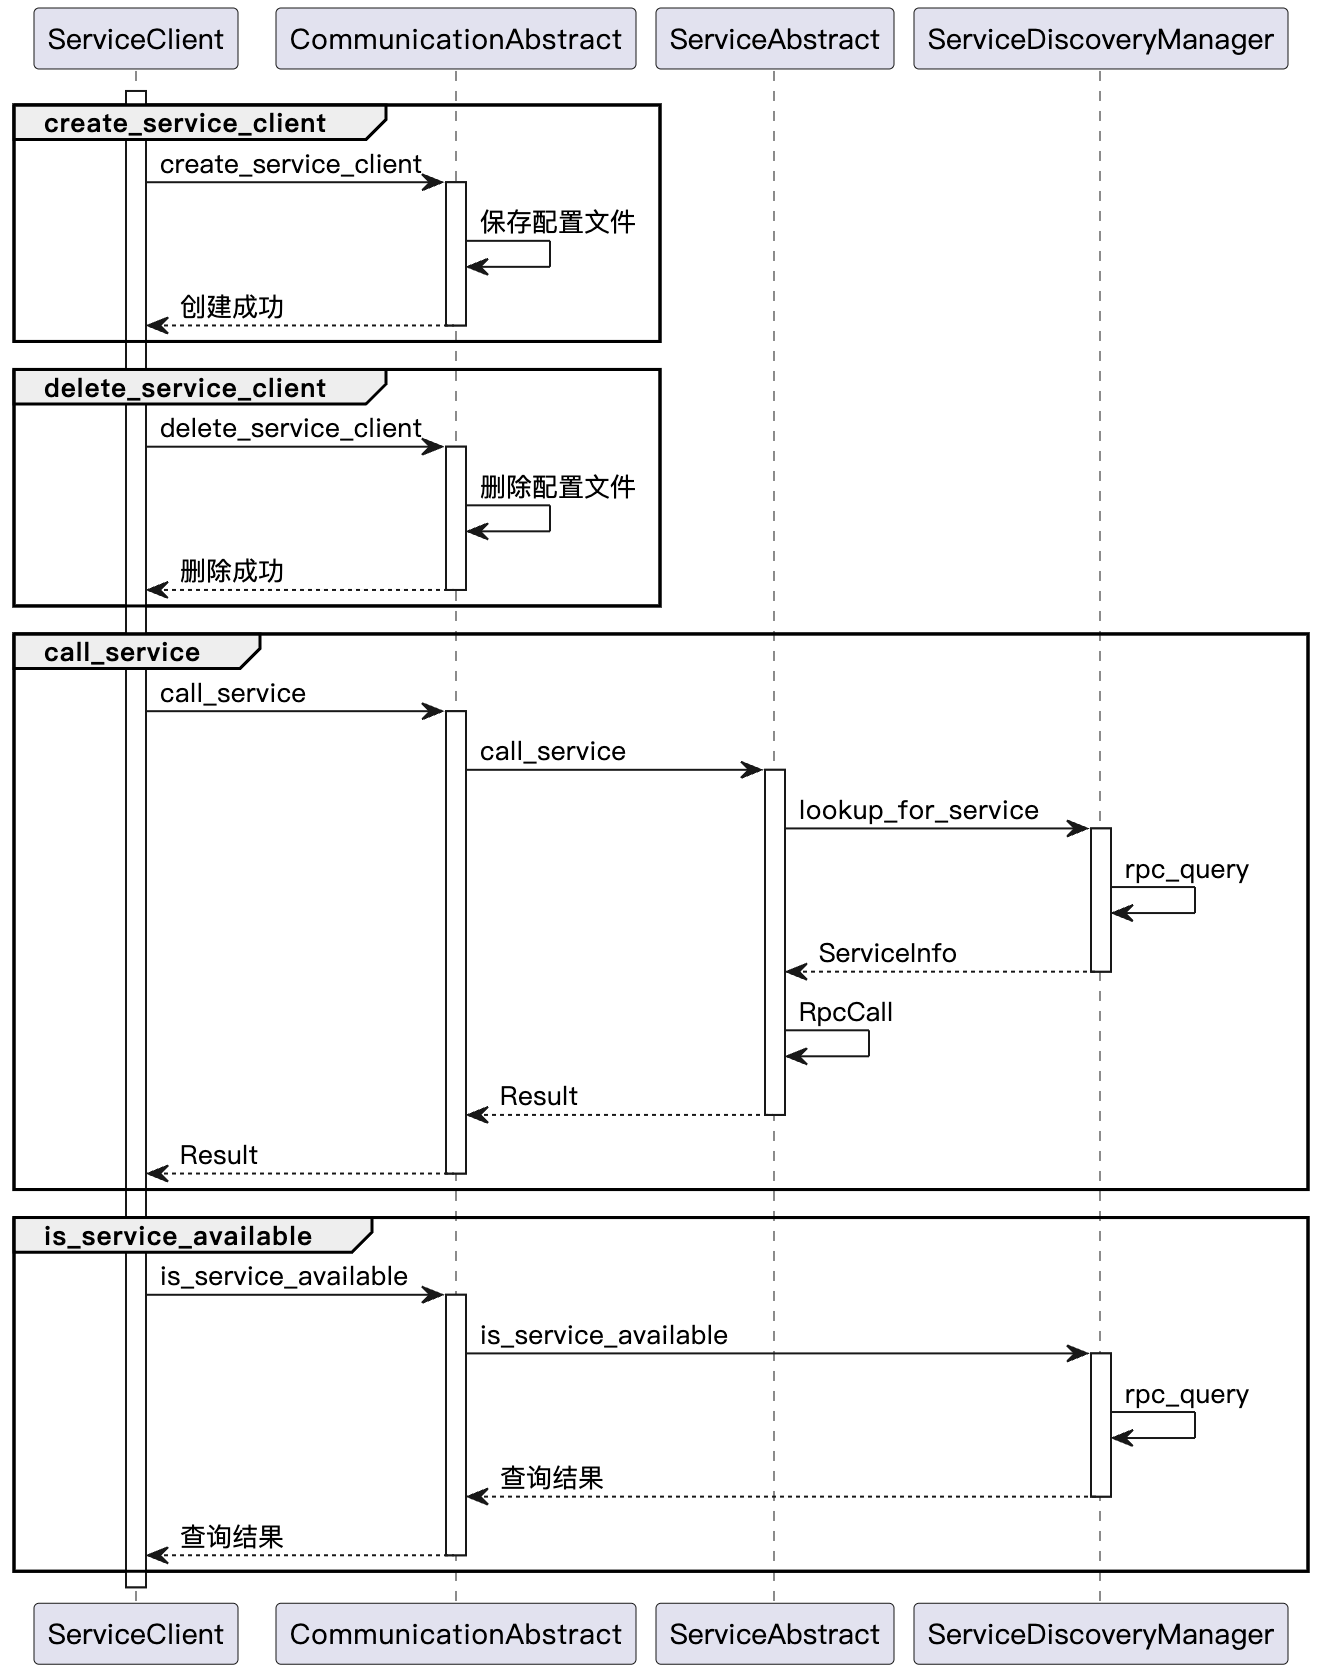
\includegraphics[width=0.85\textwidth]{5.9.png}
  \caption{客户端时序图}
  \label{client_timesequence}
\end{figure}

\section{通信抽象模块详细设计与实现}
通信抽象模块是整个通信系统承上启下的模块,一方面本模块接受通信单元模块及服务模块提供给用户的创建、删除等应用程序接口的调用,
另一方面本模块需要将用户所使用的高度抽象的应用程序接口进行处理,根据配置文件创建抽象订阅类、抽象发布类和抽象服务类并且生成服务发现请求参数通过服务发现模块
将本进程内发布者、订阅者、服务端信息更新至网络拓扑中。本模块将用户层高度抽象的接口与底层复杂的接口进行了转换。

通信抽象模块相关类设计如图\ref{communication_abstract_class}所示。通信抽象模块包含CommunicationAbstract、ServiceDiscoveryManager、PubAbstract、SubAbstract、ServiceAbstract
和Util六个类。Util类作为工具类供CommunicationAbstract类获取本机的IP地址和本进程的进程号。ServiceDiscoveryManager类提供服务发现功能。
PubAbstract、SubAbstract和ServiceAbsract三个类是本模块的核心类,三个类的生命周期CommunicationAbstract类负责。
NetworkManager(网络通信管理类)、IntraProcessManager(进程内通信管理类)和InterProcessManager(进程间通信管理类)
三个类由PubAbstract类和SubAbstract类创建并负责管理其生命周期,三个属于通信传输模块的入口类。PubAbstract类和SubAbstract类本身不实现通信的功能,而是
由内部的三个通信管理类进行实际的基于发布-订阅的通信。
ServiceAbstract类与PubAbstract类和SubAbstract类不同,内部完全实现了基于服务的通信,不需要创建额外的通信管理类辅助通信。
\begin{figure}[H]
  \centering
  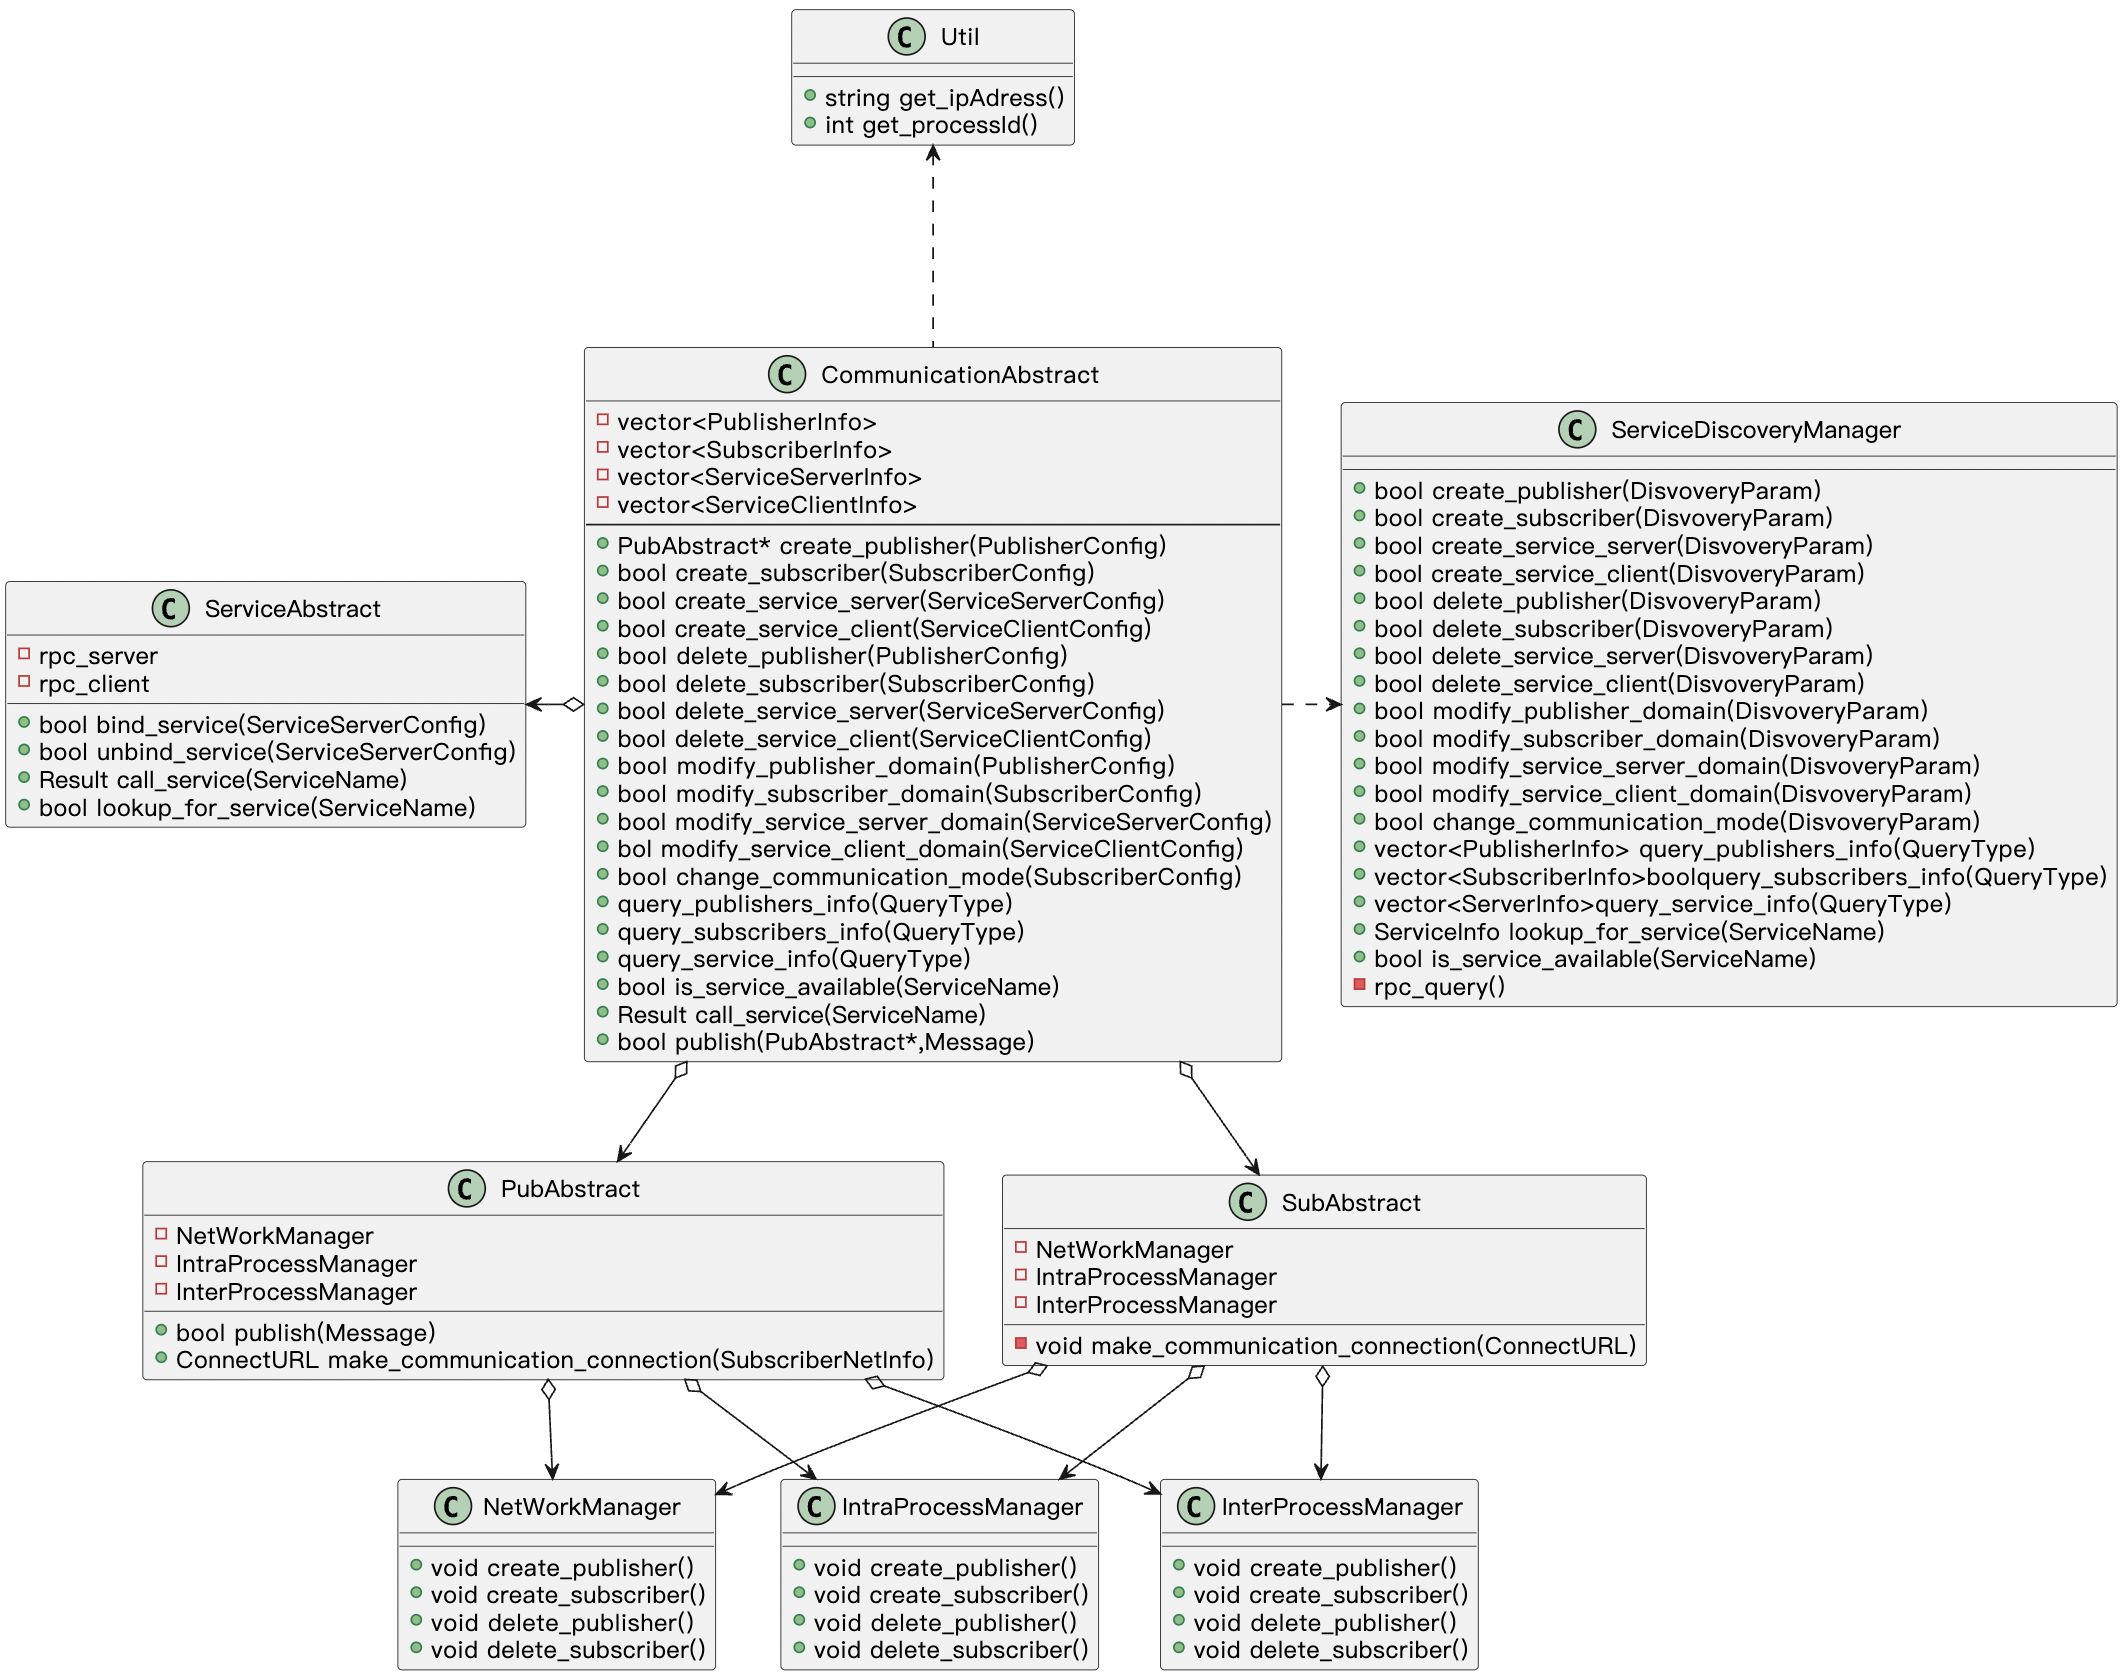
\includegraphics[width=0.95\textwidth]{5.10.png}
  \caption{通信抽象模块类图}
  \label{communication_abstract_class}
\end{figure}

本节从通信方式自适应选择算法的实现和抽象服务类的设计与实现两方面进行阐述。

\subsection{通信方式自适应选择算法实现}
本系统的核心功能之一通信方式自适应选择在本模块中的抽象发布类和抽象订阅类中的make\_communication\_connection函数实现。
根据4.4节对本模块的概要设计,通信方式自适应选择分为两部分:一部分是发布者根据自身和订阅者网络信息选择通信方式并返回连接地址,下文简称为创建算法;
另一部分是订阅者根据返回的连接地址选择通信方式并连接,下文简称为连接算法。

如算法\ref{create}所示,当发布者自身IP地址与订阅者IP不一致时返回网络通信连接地址;若IP一致但进程号不一致返回进程间
通信连接地址;若进程号一致则返回进程内通信连接地址。在返回网络地址前,使用对应的通信管理类创建发布者并将其绑定到
连接地址上。对于进程内通信和进程间通信方式,connectURL由地址前缀intraprocess或ipc加上发布者自身的话题名称组成。
对于网络通信方式,zeroMQ使用tcp为前缀的地址进行跨物理机的通信,地址中需要指定IP地址和端口号。本系统将发布者所在物理机IP
作为zeroMQ中的IP地址,端口号则设置为通配符*由zeroMQ自动寻找可用端口号。
\begin{algorithm}
  \small
  \SetAlgoLined
  \KwData{订阅者网络信息SubscriberNetInfo,发布者自身网络信息PublisherNetInfo}
  \KwResult{自适应通信连接地址,connectURL}

  \eIf{SubscriberNetInfo.ip == PublisherNetInfo.ip}{
    \eIf{SubscriberNetInfo.pid == PublisherNetInfo.pid}{
      connectURL = intraprocess://topic\_name\;
      publisher = IntraProcessManager.create\_publisher(connectURL)\;
      publisher.bind(connectURL)\;
    }{
      connectURL = ipc://topic\_name\;
      publisher = InterProcessManager.create\_publisher(connectURL)\;
      publisher.bind(connectURL)\;
    }
  }{
    connectURL = tcp://ip\_address:*\;
    publisher = NetworkManager.create\_publisher(connectURL)\;
    publisher.bind(connectURL)\;
  }
  return connectURL
  \caption{创建算法}
  \label{create}
\end{algorithm}

如算法\ref{connect}所示,订阅者得到发布者返回的连接地址后,将连接地址的前缀取出并和各通信方式连接地址的前缀比较,选择对应
的通信方式,通过对应的通信管理类创建订阅者。创建完成后调用set\_callback函数将Subscriber类中的回调函数DataCallback
注册到对应的通信管理类中并将注册的订阅者连接至连接地址上,最后通信管理类开启轮询接收消息。
\begin{algorithm}
  \small
  \SetAlgoLined
  \KwData{连接地址connectURL}
  prefix = getPrefix(connectURL)\;
  \uIf{prefix == tcp://}{
    subscriber = NetWorkProcessManager.create\_subscriber(connectURL)\;
    NetWorkProcessManager.set\_callback(DataCallback)\;
    subscriber.connect(connectURL)\;
    NetWorkProcessManager.message\_poll()\;
  }
  \uElseIf{prefix == interprocess://}{
    InterProcessManager.create\_subscriber(connectURL)\;
    InterProcessManager.set\_callback(DataCallback)\;
    subscriber.connect(connectURL)\;
    NetWorkProcessManager.message\_poll()\;

  }
  \uElseIf{prefix == intraprocess://}{
    IntraProcessManager.create\_subscriber(connectURL)\;
    IntraProcessManager.set\_callback(connectURL,DataCallback)\;
    subscriber.connect(connectURL)\;
    NetWorkProcessManager.message\_poll()\;
  }
  return 
  \caption{连接算法}
  \label{connect}
\end{algorithm}
在算法5.1和算法5.2中,抽象发布类和抽象订阅类通过三个通信管理类创建对应通信方式的发布者和订阅者,随后由通信传输模块
进行实际的消息传输,详细传输设计及算法将在下一节展开阐述,这里不做赘述。

\subsection{抽象服务类详细设计与实现}
抽象服务类内部基于rest\_rpc框架实现了基于服务的通信方式,与抽象发布类和抽象订阅类不同,该类并不需要通信抽象模块的参与即可完成通信。

从图5.10中可以看出,ServiceAbstract类存在bind\_service、unbind\_service、call\_service和lookup\_for\_service四个函数。
bind\_service函数负责绑定用户服务端提供的服务至本地rpc服务器rpc\_server中;
unbind\_service函数负责将用户需要删除的服务从本地rpc服务器中解除绑定;
call\_service函数接收用户发出的服务请求并通过rpc\_client请求服务;
lookup\_for\_service函数向服务发现模块查找需要请求的服务的IP地址;
rpc\_server和rpc\_client在ServiceAbstract类中唯一存在。

由于同一个端口只能被一个RPC服务器所监听,而服务发现模块同样需要rest\_rpc实现服务发现功能。针对此问题,
本系统在设计时将同一个进程内的ServiceAbstract类和ServiceDiscoverManager类需要提供的RPC服务绑定至同一个端口。
ServiceAbstract类内部分为两个线程,彼此之间异步地运行。一个线程用户rpc\_server接受其他客户端的服务请求,
另一个线程用于rpc\_client发起服务请求和执行bind\_service、unbind\_service、call\_service和lookup\_for\_service四个函数。
ServiceAbstract类时序图如图\ref{service_abstract_timesequence}所示。
\begin{figure}[H]
  \centering
  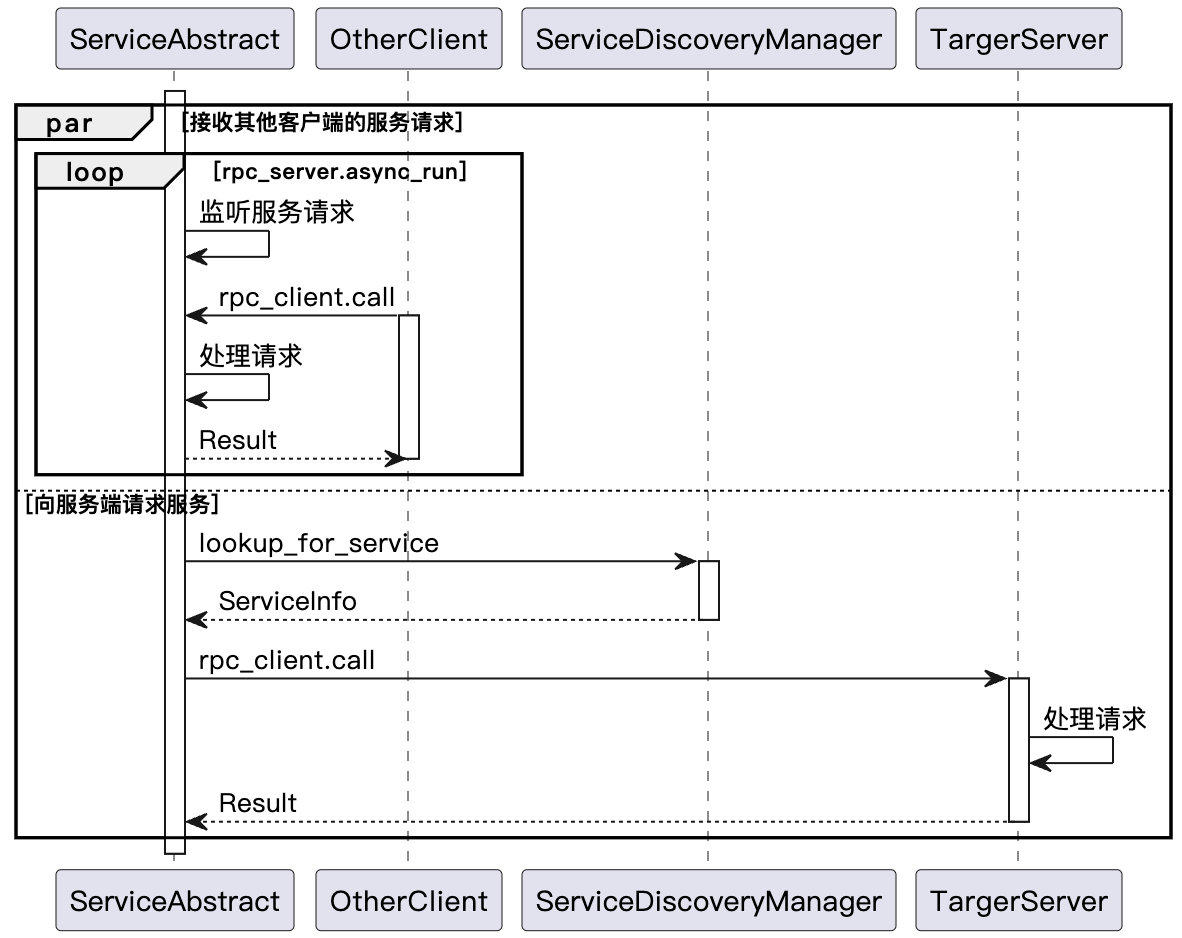
\includegraphics[width=0.85\textwidth]{5.11.png}
  \caption{抽象服务类时序图}
  \label{service_abstract_timesequence}
\end{figure}

\section{通信传输模块详细设计与实现}
通信传输模块是本系统的核心模块,基于发布-订阅的异步通信的实际消息传输全部由本模块实现。根据概要设计的设计方案,
本节将进程内通信模块、进程间通信模块、网络通信模块和消息模块进行详细设计与实现。
\subsection{进程内通信模块详细设计与实现}
根据概要设计中对本模块提出的设计方案,本模块相关类设计如图\ref{intraprocess_communication_class}所示。本模块包含进程内通信管理类IntraProcessManager、
进程内通信发布者类IntraProcessPublisher和进程内通信订阅者类IntraProcessSubscriber。IntraProcessManager类控制
IntraProcessPublisher类和IntraProcessSubscriber类的生命周期。

考虑到进程内通信并不需要严格将不同话题的发布者和订阅者区分,
IntraProcessManager类采用单例设计,每个进程中只存在一个实例,所有的进程内通信发布者和进程内通信订阅者全部保存在
IntraProcessManager类中。DataCallbacks存放所有订阅者的回调函数,根据PubAbstract类返回的connectURL完成对
不同Subscriber类中的DataCallback进行区分。
create\_publisher和create\_subscriber函数用于创建IntraProcessPublisher或IntraProcessSubscriber类。
publish函数被对应的PubAbstract类调用发布消息。
set\_callback函数被对应的SubAbstract类调用,IntraProcessManger
类将Subscriber类DataCallback与connectURL保存至哈希表DataCallbacks中。
message\_poll函数对每个IntraProcessPublisher类中的消息队列进行轮询,若有新消息则根据connectURL找到对应Subscriber类
的DataCallback执行回调函数,IntraProcessManager类中开辟新线程执行此函数。
\begin{figure}[H]
  \centering
  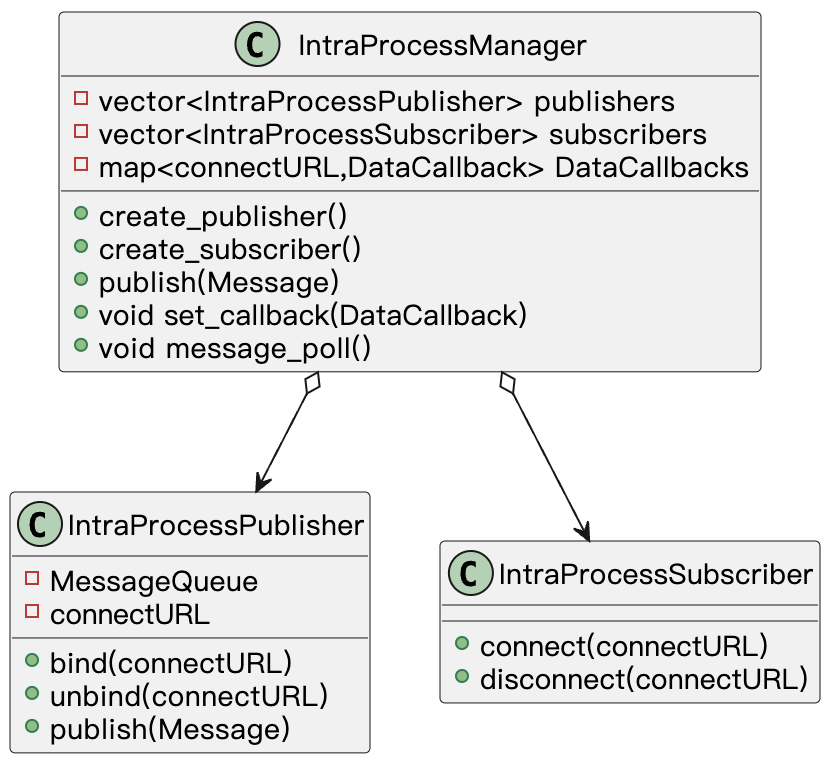
\includegraphics[width=0.65\textwidth]{5.12.png}
  \caption{进程内通信模块类图}
  \label{intraprocess_communication_class}
\end{figure}
IntraProcessPublisher类中的bind函数将IntraProcessPublisher类中的connectURL更新为PubAbstract类返回的
连接地址connectURL;unbind函数将类中的connectURL清空;publish函数将待发布消息压入类中的消息队列MessageQueue。
IntraProcessSubscriber类中的connect和disconnect函数不实现任何功能,设计这两个接口的目的是与IntraProcessPublisher类中
的bind和unbind函数相呼应。

IntraProcessManager类中message\_poll函数对消息轮询的实现如算法\ref{messagepoll}所示。如上文所述,该函数运行在
新的线程中并以死循环的方式对消息进行轮询。循环首先获取各publisher的connectURL(第3行);随后将publisher中消息队列MessageQueue
中的消息存入临时队列message(第5行);随后将该publisher的MessageQueue清空(第7行);接着在哈希表DataCallbacks中查询以connectURL键的
值是否存在(第8行);若存在根据键获取DataCallback并将临时队列所有消息作为参数调用DataCallback,将消息压入对应订阅者类Subscriber
的消息队列中并执行调度任务(第9-12行)。
\begin{algorithm}
  \small
  \SetAlgoLined
  \KwData{回调函数哈希表DataCallbacks, 进程内通信发布者publishers}
  \While{true}{
    \For{publisher in publishers}{
      connectURL = publisher.connectURL\;
      \For{message in publisher.MessageQueue}{
        messages.add(message)\;
      }
      publisher.MessageQueue.clear()\;
      bool find = DataCallbacks.find(connectURL)\;
      \If{find == true}{
        DataCallback = DataCallbacks[connectURL]\;
        \For{message in messages}{
          DataCallback(message)\;
        }
      }
    }
  }
  return 
  \caption{进程内通信消息轮询算法}
  \label{messagepoll}
\end{algorithm}

\subsection{进程间通信模块详细设计与实现}
为了改进本文第一章提到的现有自动驾驶通信系统的缺陷,进程间通信模块是本通信系统中最为复杂的一个模块。
本模块对共享内存操作使用POSIX接口(mmap、shm\_open等)实现。
本小节依次从共享内存区数据结构设计、进程间通信模块类设计以及共享内存通信机制展开论述。

\subsubsection{共享内存区数据结构设计}
本系统对共享内存区数据结构设计如图\ref{shm_data_structure}所示,共享内存区由控制和数据两部分组成。控制部分保存了该共享
内存区相关信息,而数据部分存储实际的通信消息。
\begin{figure}[H]
  \centering
  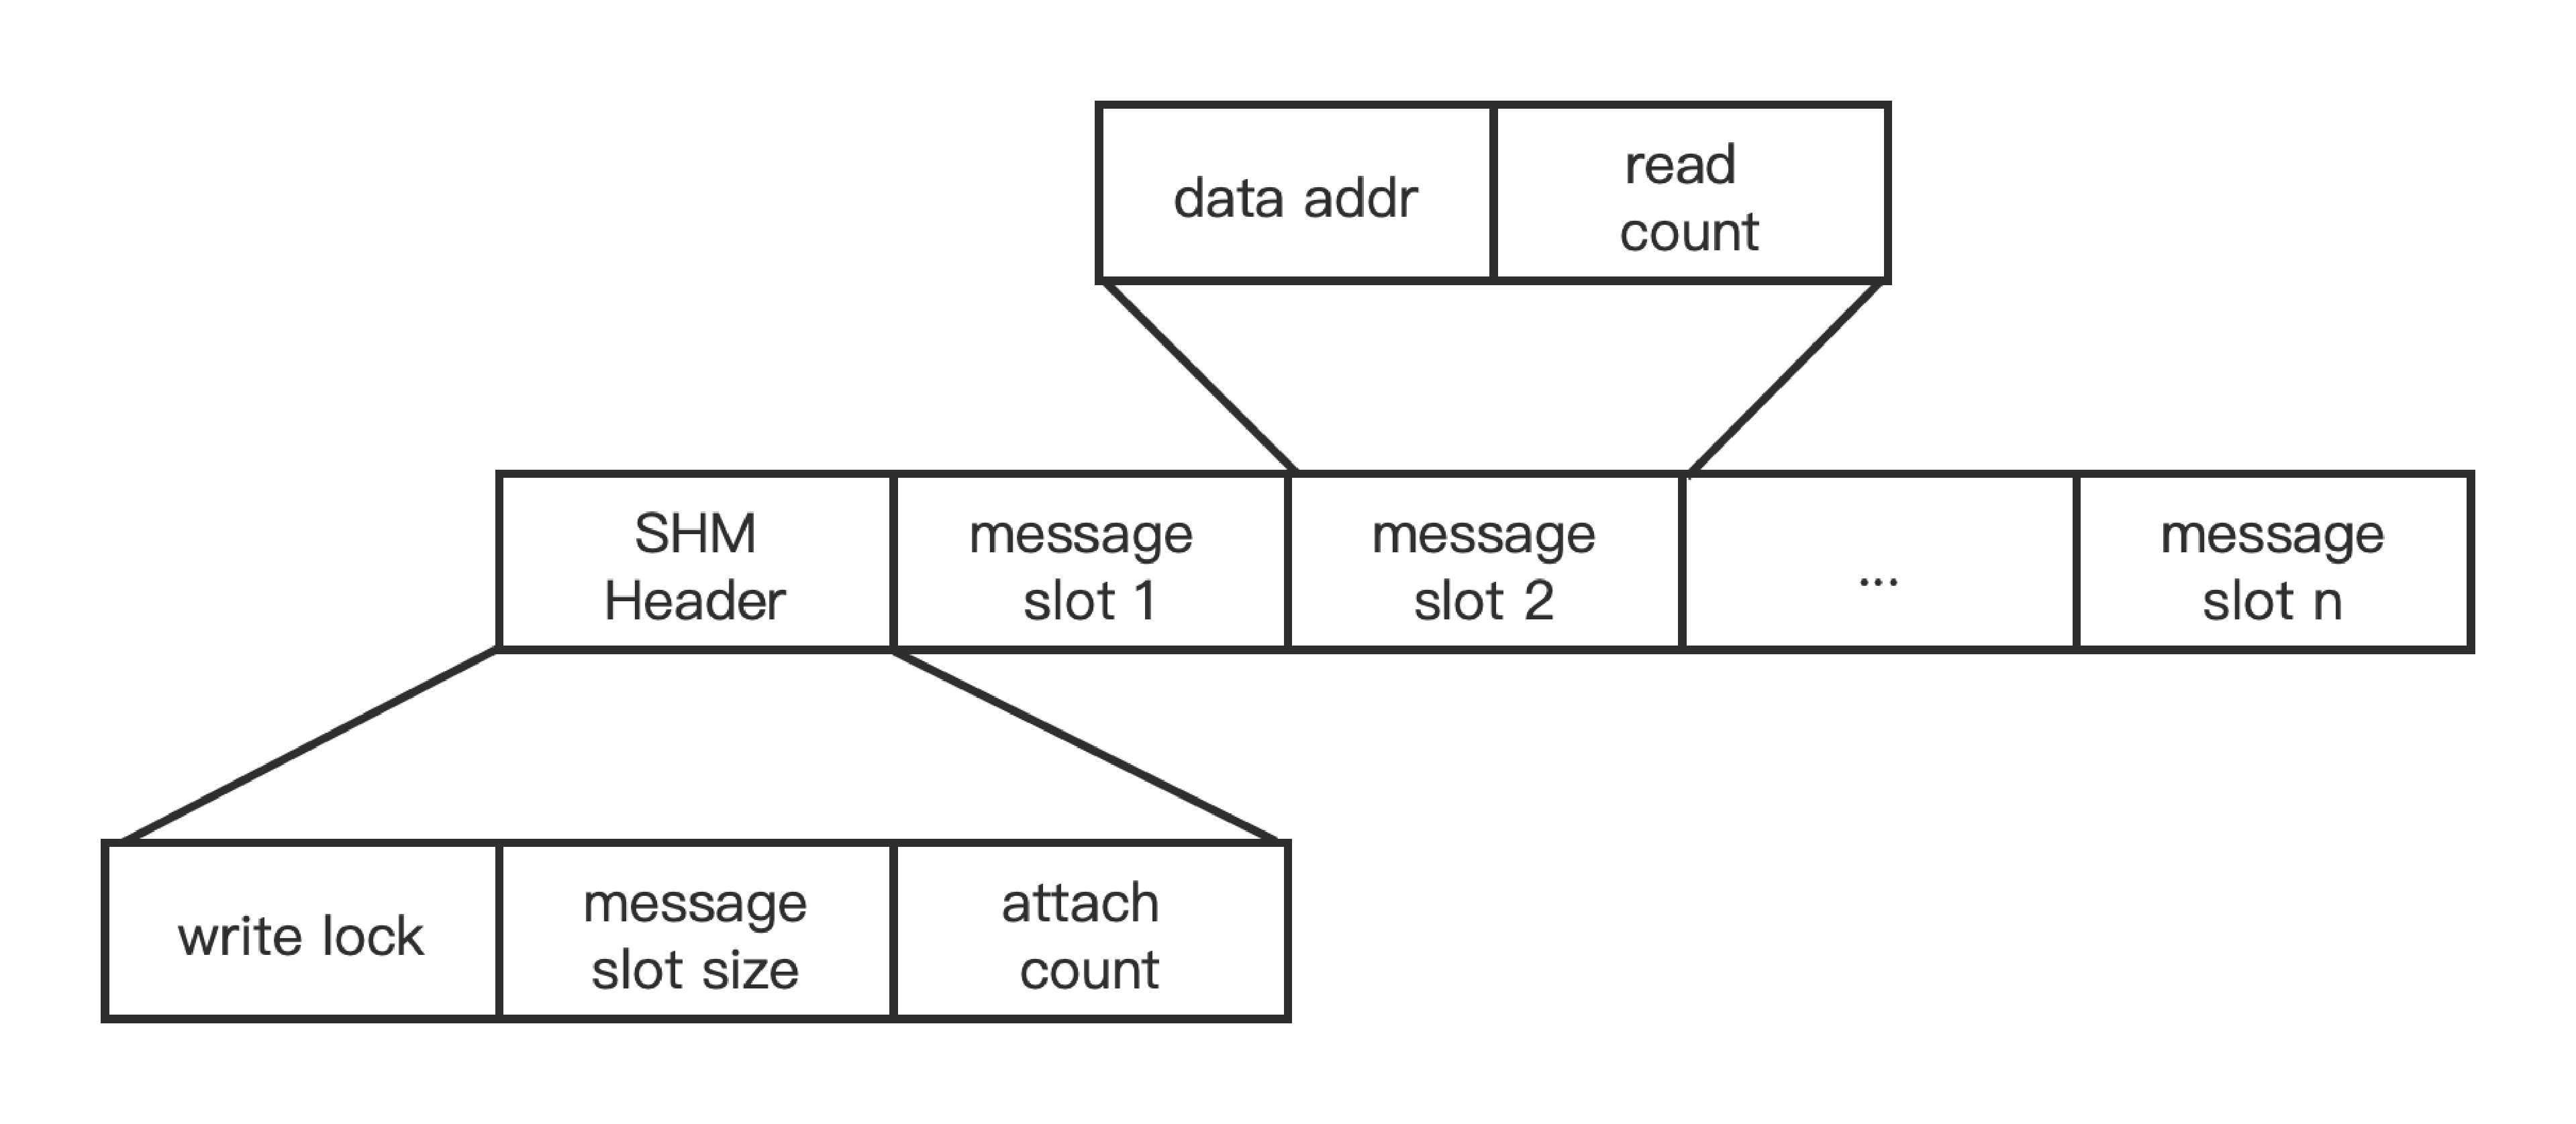
\includegraphics[width=0.85\textwidth]{5.13.pdf}
  \caption{共享内存区数据结构}
  \label{shm_data_structure}
\end{figure}

在共享内存区的控制部分SHM Header中,由write lock、message slot size、attach count三个字段对共享内存区进行实际的控制。表
5.1对SHM Header中三个字段的定义和作用作出了说明。
\begin{table}[htb]
  \centering\small
  \caption{控制部分参数说明}
  \label{tab:exampletable}
  \begin{tabular}{ccc}
    \toprule
    字段名称 & 字段类型 & 字段作用\\
    \midrule
    write lock & pthread\_mutex\_t & 保护共享内存区同一时间只能被一个发布者写入消息\\
    message slot size & int & 数据部分message slot的个数\\
    attach count & atomic\_int & 连接至共享内存区订阅者的个数\\
    \bottomrule
  \end{tabular}
\end{table}

共享内存区数据部分由多个message slot组成,message slot内部由数据地址data addr和引用计数read count组成。表5.2
对message slot中字段的定义和作用作出了说明。
\begin{table}[htb]
  \centering\small
  \caption{数据部分参数说明}
  \label{tab:exampletable}
  \begin{tabular}{ccc}
    \toprule
    字段名称 & 字段类型 & 字段作用\\
    \midrule
    data addr & uint8\_t*& 消息起始内存地址\\
    read count & atomic\_int & 当前正在读取消息的订阅者个数\\
    \bottomrule
  \end{tabular}
\end{table}

\subsubsection{进程间通信模块类设计}
根据概要设计中对本模块提出的设计方案,本模块相关类设计如图\ref{interprocess_communication_class}所示。本模块包含进程间通信管理类InterProcessManager、
进程间通信发布者类InterProcessPublisher、进程间通信订阅者类InterProcessSubscriber、共享内存写入类ShmWriter
、共享内存读取类ShmReader、共享内存区控制部分SHMReader类和共享内存区数据部分MessageSlot类。

\begin{figure}[H]
  \centering
  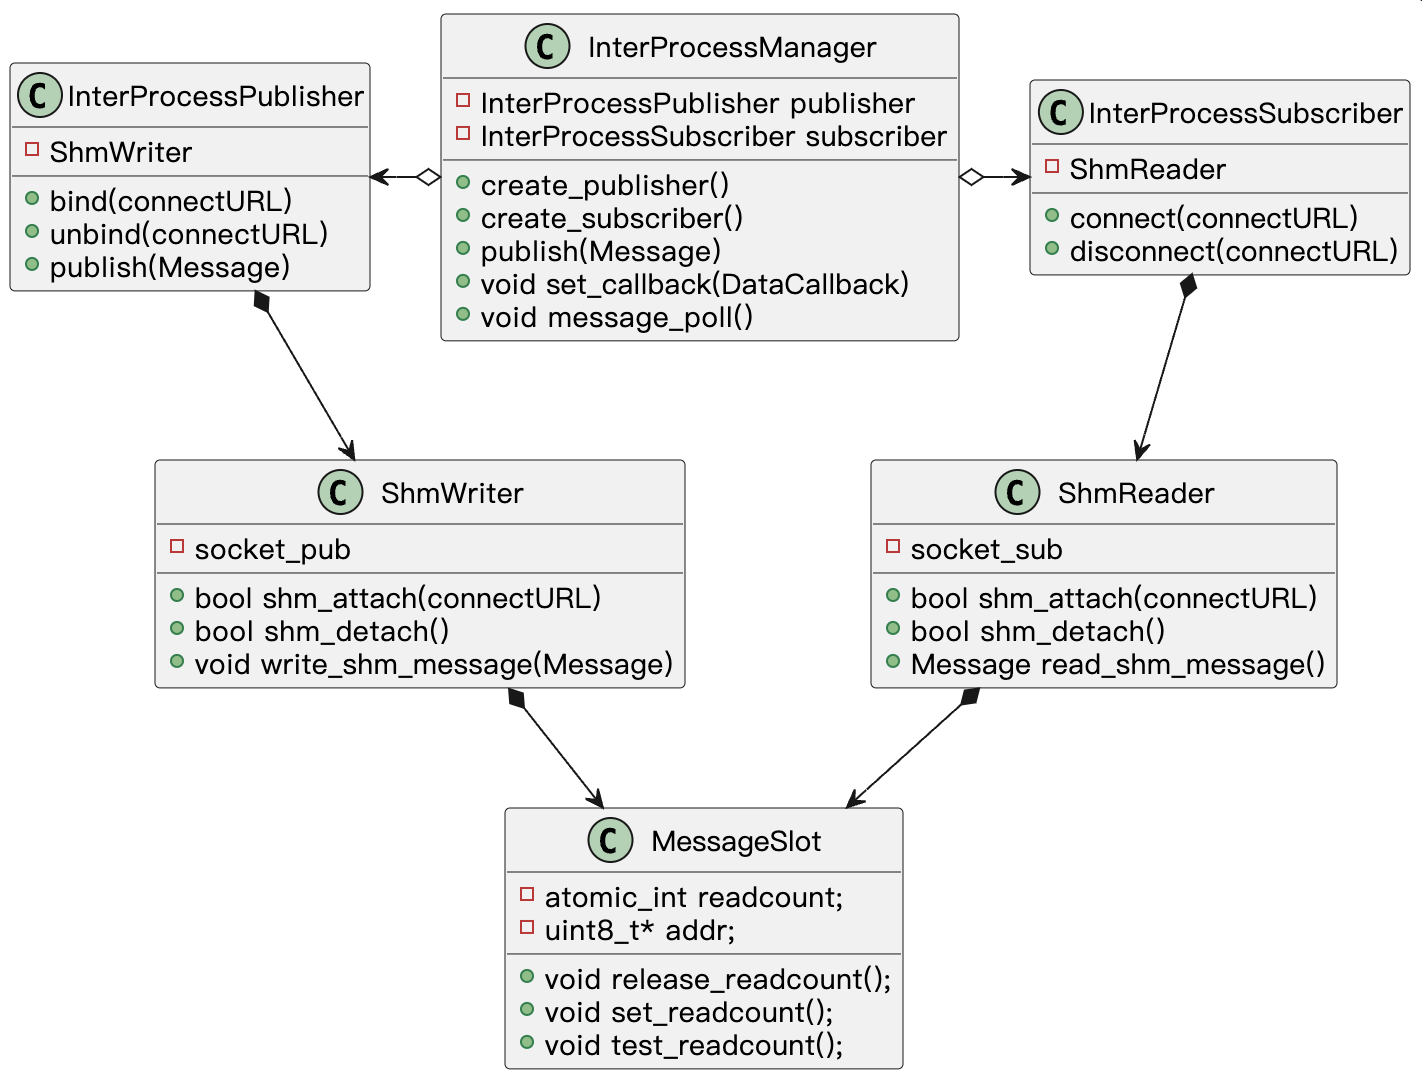
\includegraphics[width=0.75\textwidth]{5.14.png}
  \caption{进程间通信模块类图}
  \label{interprocess_communication_class}
\end{figure}
InterProcessManager类的设计与进程内通信模块中IntraProcessManager类的设计相同,InterProcessManager类
将不同话题下的发布者和通信严格区分,该类不再采用单例模设计,而是根据实际不同话题下发布者和订阅者的数量进行实例化。
同时,InterProcessManager类也不需要将Subscriber类中的DataCallback函数与connectURL一一对应并保存。

ShmWriter和ShmReader是本模块最重要的两个类,实现了向共享内存写入消息和从共享内存
读取消息的功能。如算法\ref{create}和算法\ref{connect}所示,当抽象发布类和抽象订阅类建立通信链路时,会分别调用InterProcessPublisher中的bind函数和InterProcessSubscriber
中的connect函数,随后ShmWriter与ShmReader类被创建并初始化。ShmWriter类在shm\_attach函数中根据connectURL创建
共享内存文件并在共享内存文件中初始化共享内存区数据结构,将共享内存文件地址映射至本进程的地址空间;ShmReader类
在shm\_attach函数中根据connectURL打开ShmWriter类创建的共享内存文件并将共享内存文件地址映射至本进程的地址空间。
ubind和disconnect函数将ShmWriter与ShmReader删除,ShmWriter和ShmReader通过
shm\_detach将共享内存文件与本进程解除映射。write\_shm\_message函数用于ShmWriter向共享内存中写入用户需要发布的消息并
使用网络通知各订阅者读取消息;read\_shm\_message用于ShmReader从共享内存中读取消息并通过Subscriber类中的DataCallback函数将消息压入Subscriber类中的消息队列
供用户使用。InterProcessManager通过message\_poll函数开辟新线程并轮询ShmWriter的读取通知,调用ShmReader进行
消息的读取。

SHMHeader类是共享内存区控制部分的实现,内部包含互斥锁write\_lock、message\_slot\_size和attach\_count。
write\_lock用于保护共享内存区同一时间只能被发布者占用写入消息,message\_slot\_size为数据部分message slot的个数,
attach\_count用于记录连接至共享内存区订阅者的个数。

MessageSlot类是共享内存区数据部分的实现,内部包含一个指向共享内存区域的数据首地址addr和控制
message slot中正在读取消息的订阅者个数的readcount。该类中的release\_readcount函数在ShmReader类
读取消息后被调用,函数内将readcount原子地执行减1操作。set\_readcount和test\_readcount函数被ShmWriter类
调用,set\_readcount原子地将MessageSlot类中的readcount数值置为SHMReader类中的attach\_count,test\_readcount
用于检测是否有订阅者异常退出导致readcount异常。

\subsubsection{共享内存地址规划}
由于共享内存将被映射至多个进程的地址空间中,共享内存数据结构中不能含有指向某个进程的指针,所以共享内存数据结构不能使用
C++ STL(标准模板库)中的容器是无法存放至共享内存中的,因为STL的容器会在本进程的堆空间中申请内存,对于其他进程来说
这些内存地址无法访问的。C++ Boost库(标准库的扩展)则提供了专为共享内存设计的容器,重新设计了容器的空间分配器,容器
可以被跨进程访问。但Boost库的语法比较复杂且源码体积高达1G以上,程序编译时间会明显增加,本系统不采用Boost作为共享内存通信
的实现手段。本系统采用C++中placement new的方式为共享内存数据结构分配内存,placement new的作用是在某个指定的内存地址上创建
相关变量。如图\ref{shm_addr_design}所示,共享内存数据结构各字段从mmap返回的首地址开始紧密排放,并且message\_slot中的消息起始内存地址addr
也全部为共享内存中的地址。不同进程只需要在shm\_attach函数中通过mmap返回的共享内存首地址addr即可访问SHM Header和message slot
中各变量。
\begin{figure}[H]
  \centering
  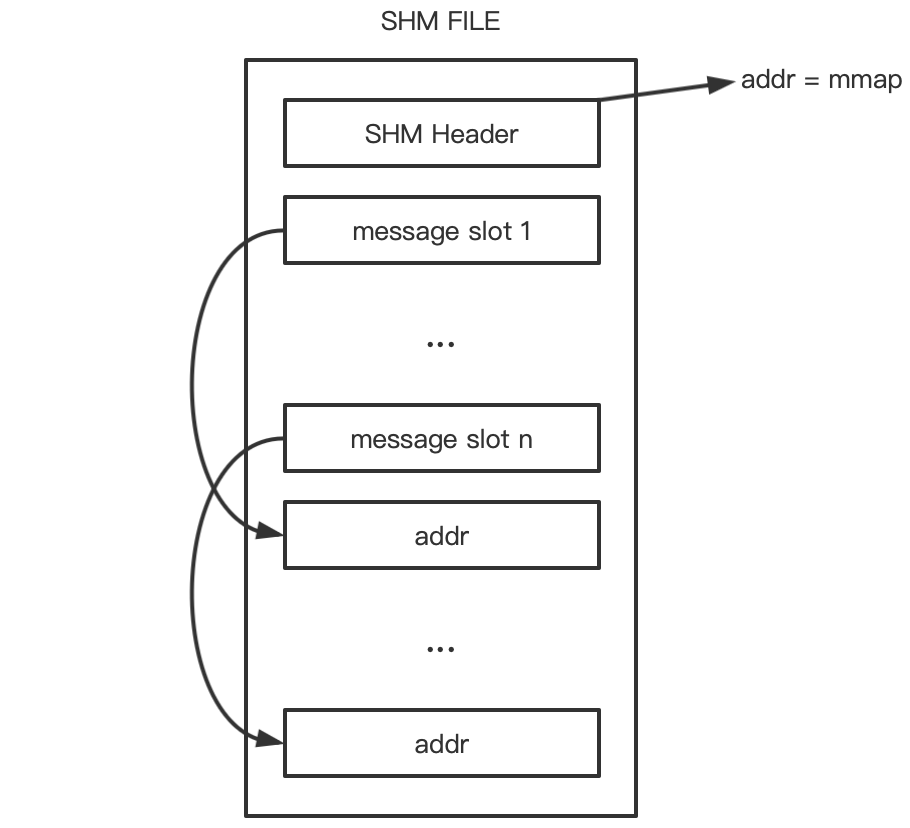
\includegraphics[width=0.6\textwidth]{5.15.png}
  \caption{共享内存地址规划}
  \label{shm_addr_design}
\end{figure}

\subsubsection{共享内存通信机制设计}
发布者首次创建共享内存区过程如算法\ref{shm_create}所示。首先通过通信话题名称topic\_name获取用于共享内存
通信的文件名称shm\_file,
\begin{algorithm}
  \small
  \SetAlgoLined
  shm\_file = shm\_ipc+topic\_name\;
  fd = shm\_open(shm\_file)\;
  addr = mmap(MAP\_SHARED,fd)\;
  SHMHeader* shm\_header = Create(addr,SHMHeader)\;
  MessageSlot* message\_slot = Create(addr+Size(SHMHeader),MessageSlot[message\_slot\_size])\;
  \For{$i \leftarrow 0$ \KwTo message\_slot\_size}{
    uint8\_t* data\_addr = Create(addr+Size(SHMHeader)+Size(MessageSlot)*message\_slot\_size\\+data\_size*i,data\_size)\;
    MessageSlot[i].data\_addr = data\_addr\;
  }
  \caption{创建共享内存区过程}
  \label{shm_create}
\end{algorithm}
使用shm\_open以及mmap函数创建共享内存文件(第1-3行);随后使用上文提到的C++ plancement new
依次将SHMHeader、MessageSlot和data\_addr创建(第4-9行)。对于SHMHeader类中类型为pthread\_mutex\_t的互斥锁write\_lock,
创建过程中SHMWriter使用pthread\_mutexattr\_setpshared函数将互斥锁write\_lock的进程共享属性设置为PTHREAD\_PROCESS\_SHARED,
使用pthread\_mutexattr\_setrobust函数将互斥锁write\_lock的健壮属性设置为PTHREAD\_MUTEX\_ROBUST。设置后,互斥锁write\_lock
可以被跨进程使用并且可以保证健壮性。
创建完成后,共享内存中的各部分地址排列如上图5.15所示。

% \begin{algorithm}[H]
%   \small
%   \SetAlgoLined
%   shm\_file = shm\_ipc+topic\_name\;
%   fd = shm\_open(shm\_file)\;
%   addr = mmap(MAP\_SHARED,fd)\;
%   SHMHeader* shm\_header = Create(addr,SHMHeader)\;
%   MessageSlot* message\_slot = Create(addr+Size(SHMHeader),MessageSlot[message\_slot\_size])\;
%   \For{$i \leftarrow 0$ \KwTo message\_slot\_size}{
%     uint8\_t* data\_addr = Create(addr+Size(SHMHeader)+Size(MessageSlot)*message\_slot\_size\\+data\_size*i,data\_size)\;
%     MessageSlot[i].data\_addr = data\_addr\;
%   }
%   \caption{创建共享内存区过程}
%   \label{shm_create}
% \end{algorithm}

发布者向共享内存中写入消息过程如算法\ref{shm_pub}所示。首先发布者请求控制部分SHM Reader中的互斥锁write\_lock取得对共享内存
区写入的权限(第1行);随后遍历数据部分MessageSlot数组查看是否存在某个MessageSlot的readcount为0,若存在则对待发布消息
Message进行序列化操作,将MessageSlot中的addr和readcount进行设置并获取序列化后消息的大小size(第2-9行);最后通过
网络方式将对应的MessageSlot下标index和消息大小size发送给订阅者通知其读取消息,释放互斥锁write\_lock(第10-11行)。

\begin{algorithm}
  \small
  \SetAlgoLined
  \KwData{待发布消息Message}
  lock(write\_lock)\;
  \For{$index \leftarrow 0$ \KwTo message\_slot\_size}{
    \If{MessageSlot[index].readcount == $0$}{
      MessageSlot[index].addr = Serialize(Messsage)\;
      size = Size(Message)\;
      set\_readcount(MessageSlot[index].readcount)\;
      break\;
    }
  }
  socket.send(index,size)\;
  unlock(write\_lock)\;
  \caption{进程间通信发布消息过程}
  \label{shm_pub}
\end{algorithm}

订阅者从共享内存中读取消息过程如算法\ref{shm_sub}所示。首先订阅者根据下标index获取对应MessageSlot中的数据首地址addr(第1行);
随后通过首地址addr和数据大小size将序列化后的消息存入buf并进行反序列化(第2-3行);序列化完成后将readcount原子地减1(第4行);
最后调用DataCallback函数将消息压入Subscriber类中的消息队列并激活调度任务(第5行)。

\begin{algorithm}
  \small
  \SetAlgoLined
  \KwData{Socket Message(index,size)}
  addr = MessageSlot[index].addr\;
  buf = copy(addr,size)\;
  Message = DeSerialize(buf)\;
  release\_readcount()\;
  DataCallback(Message)\;

  \caption{进程间通信订阅消息过程}
  \label{shm_sub}
\end{algorithm}

当多个发布者中的一个或多个由于异常退出无法正常释放互斥锁write\_lock导致其他发布者无法再次取得互斥锁的情况,本模块使用
pthread\_mutexattr\_setrobust函数将互斥锁write\_lock设置为PTHREAD\_MUTEX\_ROBUST属性,被多个发布者共享的
互斥锁拥有健壮性。当某个发布者尚未释放获得的互斥锁异常退出后,其他发布者使用pthread\_mutex\_lock函数再次尝试获取互斥锁时
会返回EOWNERDEAD的错误码,只需要调用pthread\_mutex\_consistent函数恢复互斥锁的一致性即可正常使用。

当订阅者发生异常退出无法正常释放message slot中的readcount时,本模块并不会立即采取恢复readcount一致性的操作。
根据算法\ref{shm_pub}发布者向共享内存中写入消息会查找第一个readcount等于零的message slot,当发布者无法找到满足
条件的message slot时,会调用test\_readcount函数对每一个message slot中的readcount进行检查。检查算法如算法\ref{shm_test}
所示。首先定义订阅者异常退出数量kdump\_count(第1行);随后遍历共享内存区数据部分中所有MessageSlot类,使用原子操作CAS尝试将其中的readcount置0,
若尝试次数超过10次则将该readcount与kdump\_count取较大值并赋值给kdump\_dump(第4-10行);最后使用原子操作将共享
内存区控制部分SHMHeader中的attach\_count减去异常退出的订阅者数量(第12行)。执行完test\_readcount函数后,SHMHeader
中的attach\_count与实际连接至共享内存订阅者数量恢复一致。
\begin{algorithm}
  \small
  \SetAlgoLined
  \KwData{MessageSlot}
  kdump\_count = 0\;
  \For{$index \leftarrow 0$ \KwTo message\_slot\_size}{
    try\_times = 0\;
    \While{MessageSlot[index].readcount.CAS(0,0) not true}{
      try\_times++\;
      \If{try\_times > 10}{
        kdump\_count = max(kdump\_count,MessageSlot[index].readcount)\;
        break\;
      }
    }
  }
  SHMHeader.attach\_count.fetch\_sub(kdump\_count)\;
  \caption{订阅者崩溃检测}
  \label{shm_test}
\end{algorithm}

\subsection{网络通信模块详细设计与实现}
根据概要设计中对本模块提出的设计方案,本模块相关类设计如图\ref{network_communication}所示。本模块包含网络通信
管理类NetworkManager、网络通信发布者类NetworkPublisher和网络通信订阅者类NetworkSubscriber。NetworkManager类
控制NetworkPublisher类和NetworkSubscriber类的生命周期。

NetworkPublisher类中包含一个未初始化的ZeroMQ套接字zmq\_socket,在算法\ref{create}抽象发布类PubAbstract创建NetworkPublisher类实例后会调用
该类内部的bind函数,函数中将zmq\_socket套接字初始化为ZMQ\_PUB属性并绑定至connectURL。

NetworkSubscriber类中同样包含一个未初始化的ZeroMQ套接字zmq\_socket,在算法\ref{connect}抽象订阅类SubAbstract
创建NetworkSubscriber类实例后调用该类内部connect函数,函数中将zmq\_socket套接字初始化为ZMQ\_SUB属性并连接至connectURL。
\begin{figure}[H]
  \centering
  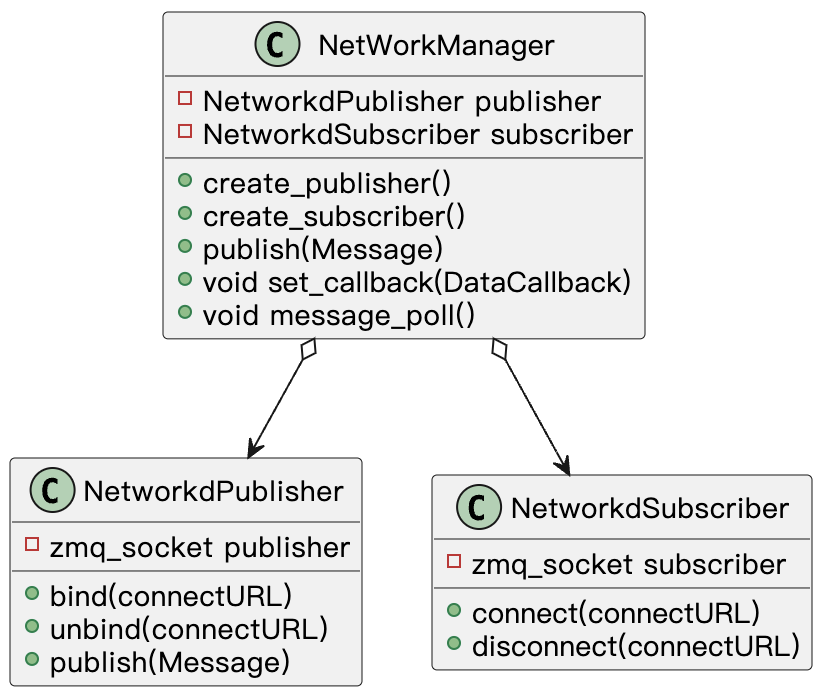
\includegraphics[width=0.65\textwidth]{network_communication.png}
  \caption{网络通信模块类图}
  \label{network_communication}
\end{figure}
NetworkManager类开辟新线程执行message\_poll,函数内部以死循环的方式对消息进行轮询,具体实现如算法\ref{network_messagepoll}所示。
首先定义ZeroMQ的消息变量message(第2行);随后使用subscriber类中的zmq\_socket接收消息并进入阻塞状态,直至接收到publisher发布的
ZeroMQ消息(第3行);接收到消息后,对消息进行反序列化(第4行);最后将消息作为参数调用DataCallback,将消息压入对应订阅者类Subscriber
的消息队列中并执行调度任务(第5行)。
\begin{algorithm}
  \small
  \SetAlgoLined
  \KwData{ZeroMQ message}
  \While{true}{
    zmq\_message message\;
    subscriber.zmq\_socket.recv(message)\;
    Message = DeSerialize(message)\;
    DataCallback(Message)\;
  }
  return 
  \caption{进程内通信消息轮询算法}
  \label{network_messagepoll}
\end{algorithm}

\subsection{消息模块详细设计与实现}
消息模块模块作为网络通信模块和进程间通信模块的中间模块,该模块将C++原生数据结构与Google Protobuf进行抽象处理,
为两个通信模块提供消息的序列化功能与反序列功能。

本模块通过用户编写的.proto文件,通过C++构建工具CMake和python自动生成一套介于C++原生数据结构和protobuf数据结构之间
的中间语言。中间语言生成的过程如图\ref{middle_language_flowchart}所示。
\begin{figure}[H]
  \centering
  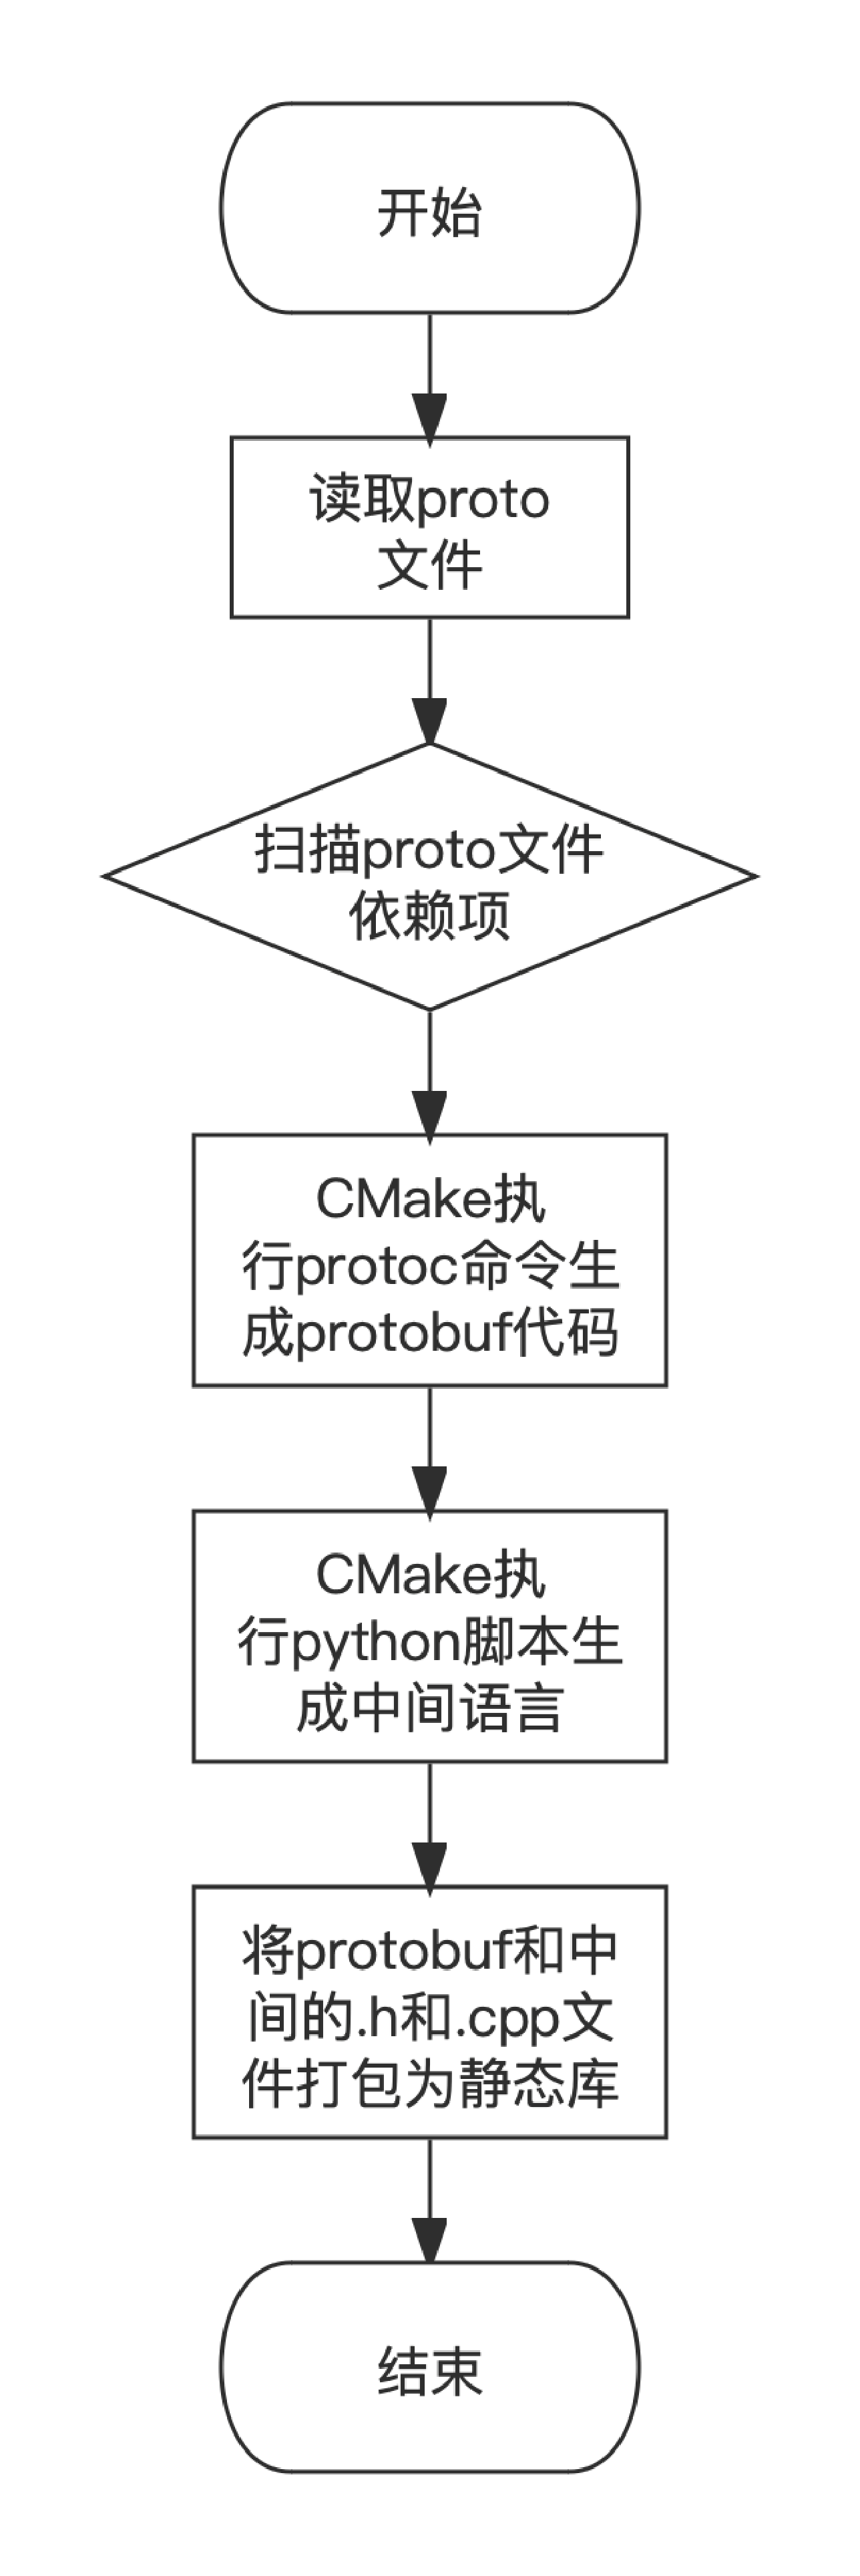
\includegraphics[width=0.25\textwidth]{middle_language_flowchart.pdf}
  \caption{中间语言生成流程图}
  \label{middle_language_flowchart}
\end{figure}
生成protobuf代码以及中间语言全部在通过构建工具CMake提供的EXECUTE\_PROCESS命令完成,首先通过该命令调用protobuf提供的
protoc工具生成protobuf代码。随后继续使用EXECUTE\_PROCESS执行python脚本生成中间语言。

python脚本首先读取目录下所有用户编写完成的.proto文件并扫描依赖项,若某个.proto文件依赖其他.proto文件则生成依赖图。
扫描完成后,脚本内部得到所有.proto文件的字段名及其数据类型,脚本表\ref{type_convert}生成protobuf数据类型和C++数据类型
的字典。中间语言预设了C++ .h文件与.cpp文件的模板,python脚本生成数据类型字典后开始逐一生成.h文件与.cpp文件中的
保留字段,保留字段包括头文件引用、消息类函数的声明、类函数的实现等。
\begin{table}[htb]
  \centering\small
  \caption{类型转换表}
  \label{type_convert}
  \begin{tabular}{cc}
    \toprule
    Protocol Buffer & C++ \\
    \midrule
    bool & bool \\
    int32 & int32\_t \\
    int64 & int64\_t \\
    uint32 & uint32\_t \\ 
    uint64 & uint64\_t \\
    float & float \\
    double & double \\
    string & std::string \\
    repeated Type & std::vector<Type>\\
    \bottomrule
  \end{tabular}
\end{table}

本节以Example消息为例阐述中间语言消息类的构成,Example生成的中间语言消息类的类图如图\ref{middle_language_class}所示。
本模块生成的所有中间语言消息类全部继承抽象消息类AbstractMessage,该类中定义了四个虚函数。serialized\_data\_bytes函数用于
获取序列化后数据的大小;serialized函数用于序列化数据;deserialized函数用于反序列化数据;conver函数用于C++数据类型和protobuf数据类型
的互换。ExampleMessage类实现AbstractMessage所有虚函数并在类内部定义protobuf生成的Example类实例,通过该实例
与protobuf进行序列化与反序列化的交互。
\begin{figure}[H]
  \centering
  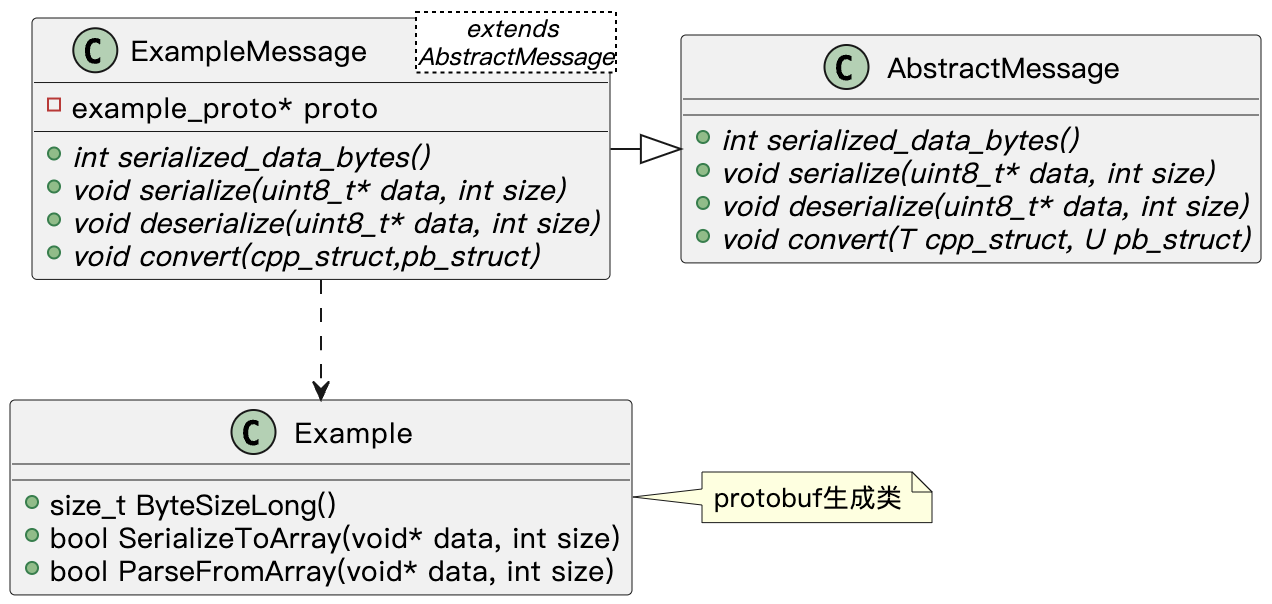
\includegraphics[width=0.8\textwidth]{middle_language_class.png}
  \caption{中间语言消息类图}
  \label{middle_language_class}
\end{figure}
图\ref{middle_language_class}仅展示了一个消息类的构成,实际运用中会存在少则几十多则上百种不同的消息。本模块
为了便于用户使用,将所有中间语言和protobuf生成的.cpp统一生成静态库,用户只需要引用对应消息的头文件和链接静态库即可将所有
处理消息的函数符号导入到程序中。













\section{服务发现模块详细设计与实现}
服务发现模块是通信系统与中心节点交换网络信息的重要模块,本模块与中心节点通过RPC形式进行网络拓扑信息的交互控制通信链路并
向用户提供查询网络拓扑信息功能。

\subsection{服务发现模块类设计}
服务发现模块相关类如图\ref{service_discovery_class}所示,本模块类构成相对简单,包含ServiceDiscoveryManager、rpc\_client、rpc\_server
三个类。rpc\_client类和rpc\_server类由C++ RPC框架rest\_rpc实现,提供最基本的服务绑定与请求功能。
ServiceDiscoveryManager类采用单例设计模式,
使用rest\_rpc框架完成与中心节点的网络拓扑信息交互并控制通信链路,所有函数均由CommunicationAbstract通信抽象类
和ServiceAbstract抽象服务类调用。ServiceDiscoveryManager类的内部保存本进程内所有发布者、订阅者、服务客户端和服务服务端的信息,即PublisherInfo、
SubscriberInfo、ServiceClientInfo和ServiceServerInfo。

\begin{figure}[htb]
  \centering
  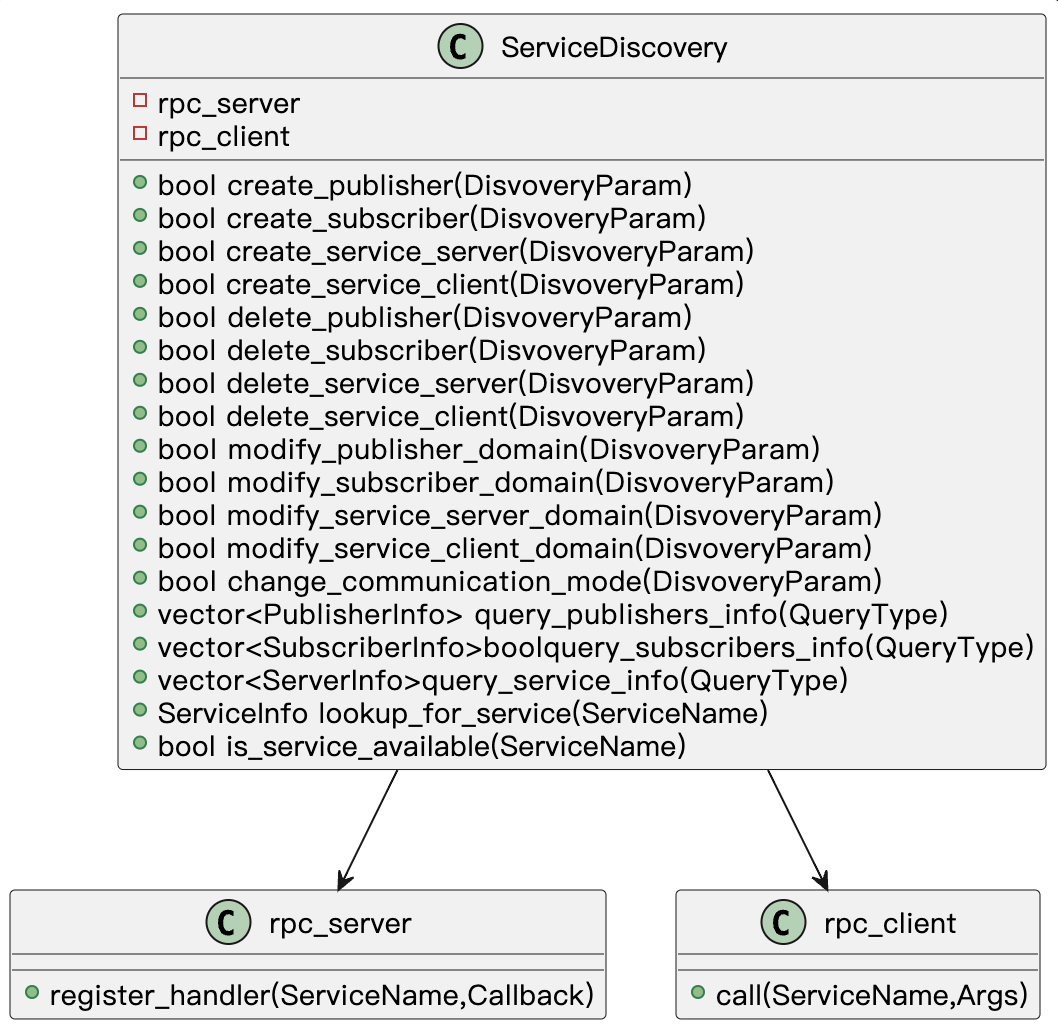
\includegraphics[width=0.7\textwidth]{5.16.png}
  \caption{服务发现模块类图}
  \label{service_discovery_class}
\end{figure}

ServiceDiscoveryManager类被实例化时会调用自身内部的start函数将本模块RPC通信地址(IP地址与端口号)通过RPC形式通知中心节点,
随后执行init\_service函数绑定服务接收来自中心节点的信息查询请求。初始化完成后ServiceDiscoveryManager类一方面接受来自
CommunicationAbstract通信抽象类和ServiceAbstract抽象服务类的主动调用,上传自身网络拓扑信息至中心节点;另一方面,ServiceDiscoveryManager类
接受来自中心节点的更新信息查询请求。


\subsection{发现机制设计}
概要设计中,服务发现模块发现机制分为主动发现与被动发现两类。主动发现机制分为如下三情况:
\begin{enumerate}
  \item 当注册、删除或修改发布者和订阅者时,ServiceDiscoveryManager类构造请求信息向中心节点发出RPC调用获取匹配通信方后,根据自身保存的
  更新通信链路回调函数Callback,调用PubAbstract类和SubAbstract类中的make\_communication\_connection函数建立通信链路,并将连接地址和订阅者信息通过RPC方式发送至其他关联的服务发现模块。
  \item 当注册、删除或修改服务服务端时,ServiceDiscoveryManager类只向中心节点更新服务端的IP和端口信息。
  \item 当注册、删除或修改服务客户端时,ServiceDiscoveryManager类不向中心节点更新客户端的信息,只有当客户端通过ServiceAbstract类发出实际请求时ServiceDiscoveryManager类
  根据服务名向中心节点查询服务端的IP和端口信息返回至ServiceAbstract类。
\end{enumerate}
以注册发布者为例,服务发现模块与中心节点之间的信息流向如图\ref{service_discovery_message_flow}所示。

\begin{figure}[H]
  \centering
  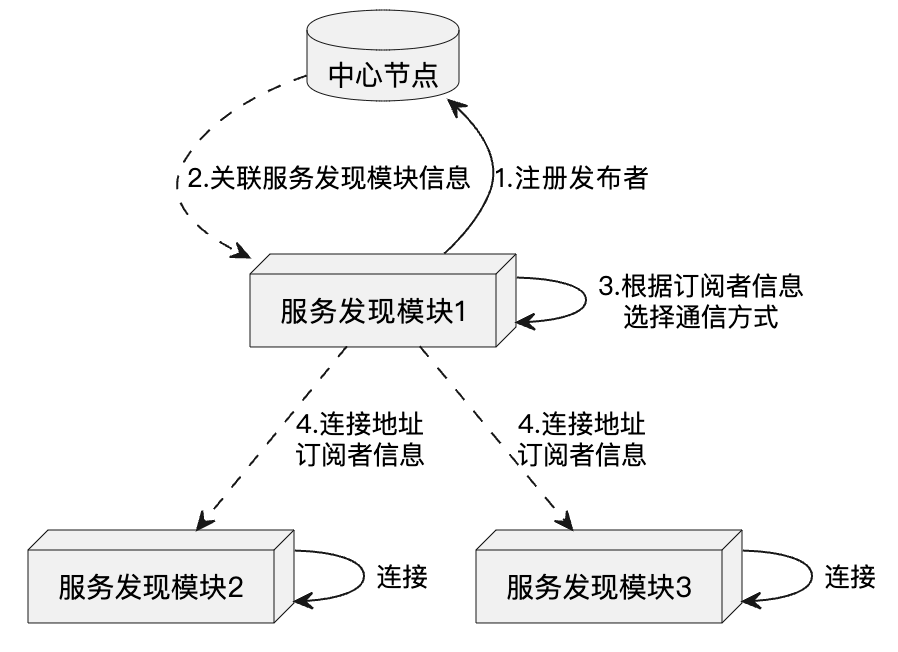
\includegraphics[width=0.7\textwidth]{5.17.png}
  \caption{服务发现信息流向图}
  \label{service_discovery_message_flow}
\end{figure}

被动发现机制并不由用户的操作触发,而是由ServiceDiscoveryManager类在初始化中通过rest\_rpc注册供中心节点调用的服务。被动
发现机制提供的服务如下:
\begin{enumerate}
  \item 更新发布者:其他进程注册、删除或修改发布者时,将创建的连接地址和订阅者信息通过RPC方式发送本进程。ServiceDiscoveryManager类
  根据订阅者信息中的话题名称Topic找到对应的SubscriberInfo,通过其中的Callback调用SubAbstract类的make\_communication\_connection函数
  选择对应的通信方式。
  \item 更新订阅者:其他进程注册、删除或修改订阅者时,中心节点会将其他进程服务发现模块的RPC地址和订阅者信息通过RPC方式发送至本进程。
  ServiceDiscoveryManager类根据订阅者话题名称Topic找到对应的PublisherInfo,通过其中的Callback调用PubAbstract类的make\_communication\_connection函数
  选择对应的通信方式,最后将连接地址和订阅者信息返回至其他进程的服务发现模块。
\end{enumerate}

\section{任务模块详细设计与实现}
任务模块本身并不提供功能逻辑,功能模块的作用是向用户提供一个统一的基类,
用户需要继承基类并创建具体的任务类。根据概要设计中的设计方案,任务模块类设计如图\ref{task_class}所示。
\begin{figure}[H]
  \centering
  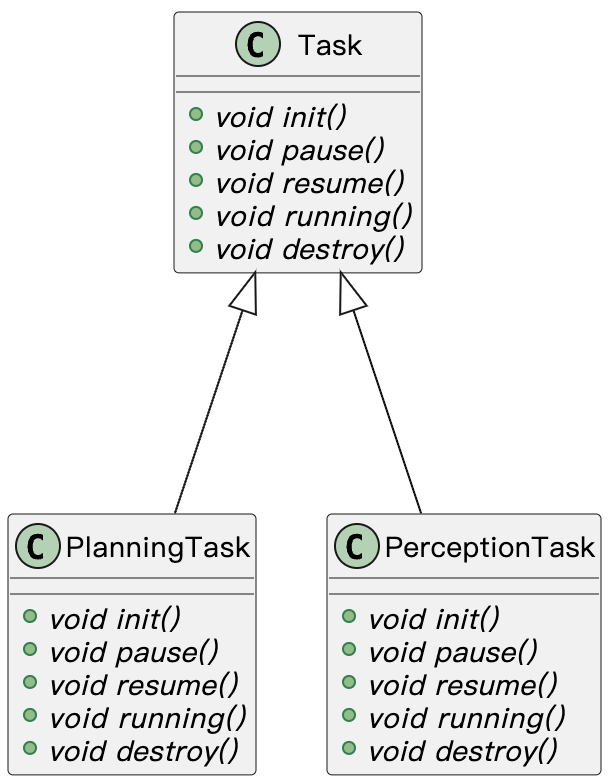
\includegraphics[width=0.4\textwidth]{5.18.png}
  \caption{任务模块类图}
  \label{task_class}
\end{figure}
任务模块的基类Task中的init、pause、resume、running和destroy五个函数全部为纯虚函数,内部不实现任何逻辑。
用户需要定义自身的任务类如图5.12中的规划任务(PlanningTask)和感知任务(PerceptionTask)继承基类,并
实现五个函数的逻辑功能。

\section{调度模块详细设计与实现}
调度模块使用基于消息触发和基于时间触发两种策略调度控制用户任务的运行,调度模块类图设计如图\ref{schedul_class}所示。
Scheduler类采用单例设计,每个进程中只存在一个实例。TaskEntity是调度实体,由任务名TaskName、任务回调函数TaskCallback
以及缓冲队列Buffer构成,TaskEntity与调度任务一一对应,本系统规定TaskEntity中的回调函数必须是用户任务中的
running函数。
create\_message\_task与create\_time\_task函数
分别向Scheduler类注册基于消息触发的调度任务和基于时间触发的调度任务。activate\_task函数用于激活基于消息触发
的调度任务。start\_schedule函数用于开始任务的调度,将start置为true,所有调度任务都需要start为true时才会
执行调度任务。
\begin{figure}[H]
  \centering
  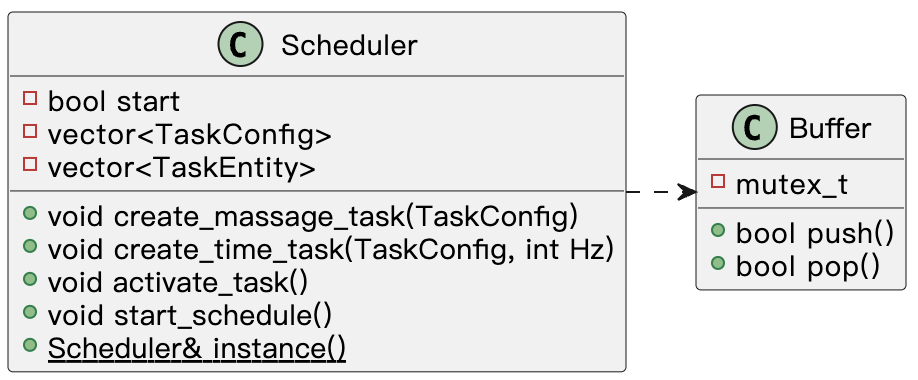
\includegraphics[width=0.65\textwidth]{5.19.png}
  \caption{调度模块类图}
  \label{schedul_class}
\end{figure}

\subsection{基于消息触发的调度详细设计与实现}
根据概要设计的设计,基于消息触发的调度策略是侵入式的,即该调度策略并不需要用户手动地配置TaskEntity中的各字段,
而是在Subsciber类被实例化时自动填充TaskEntity各字段并调用create\_message\_task函数注册调度任务。
注册调度任务成功后,将activate\_task函数与Subscriber类的DataCallback回调函数生成新的回调函数DataCallback。
当有新消息到来时通信新的回调函数DataCallback被执行,函数中先将消息压入消息队列随后激活调度任务行用户任务中的running函数。激活调度任务并不直接调用
任务回调函数TaskCallback,而是将对应任务的缓冲队列Buffer中压入一个元素。

当调用create\_message\_task函数注册任务后,Scheduler类会将每一个基于消息触发调度策略的任务开辟一个新的线程,
线程中采用死循环判断缓冲队列是否不为空,若不为空则调用TaskEntity中的TaskCallback激活任务,否则继续判断直到缓冲队列不为空。
每个调度任务运行在不同的线程中。

\subsection{基于时间触发的调度详细设计与实现}
基于时间触发的调度策略不再是侵入式,而是需要用户手动设定TaskEntity中各字段并设定调度频率,调度频率单位是赫兹(Hz)。
当用户调用create\_time\_task函数后Scheduler类会开辟一个新的线程并开始以固定的频率执行用户任务中的running函数。
该调度策略最重要的是如何将用户任务中的running(TaskCallback)函数尽可能贴合用户设置的调度频率。针对此问题,本小节给出的实现
如算法\ref{scheduler}所示。Scheduler类的开辟新的线程后,使用C++中ratio库计算调度的间隔(第1行);随后进入死循环,
获取执行TaskCallback函数之前的时间点start(第3行);当TaskCallback运行结束后再次获取时间点end并计算
运行耗时cost(第4-6行);随后计算需要等待的时间wait(第7行);如果等待时间小于0则直接进行下一次调度,否则线程睡眠(第8-11行)。

\begin{algorithm}[H]
  \small
  \SetAlgoLined
  \KwData{调度频率$Hz$}
  duration = ratio(1,Hz)\;
  \While{true}{
    clock start = now\;
    TaskCallback\;
    clock end = now\;
    clock cost = end - start\;
    clock wait = duration - cost\;
    \uIf {wait <= 0}{
      continue\;
    }
    \Else{
      sleep(wait)\;
    }
  }
  \caption{时间触发调度算法}
  \label{scheduler}
\end{algorithm}

整个任务调度模块的线程运行如图\ref{thread_running}所示。消息调度线程只有当Subscriber类中的回调函数DataCallback被抽象订阅类调用是
才会被激活并执行TaskCallback,而时间调度线程以固定频率执行TaskCallback。
\begin{figure}[H]
  \centering
  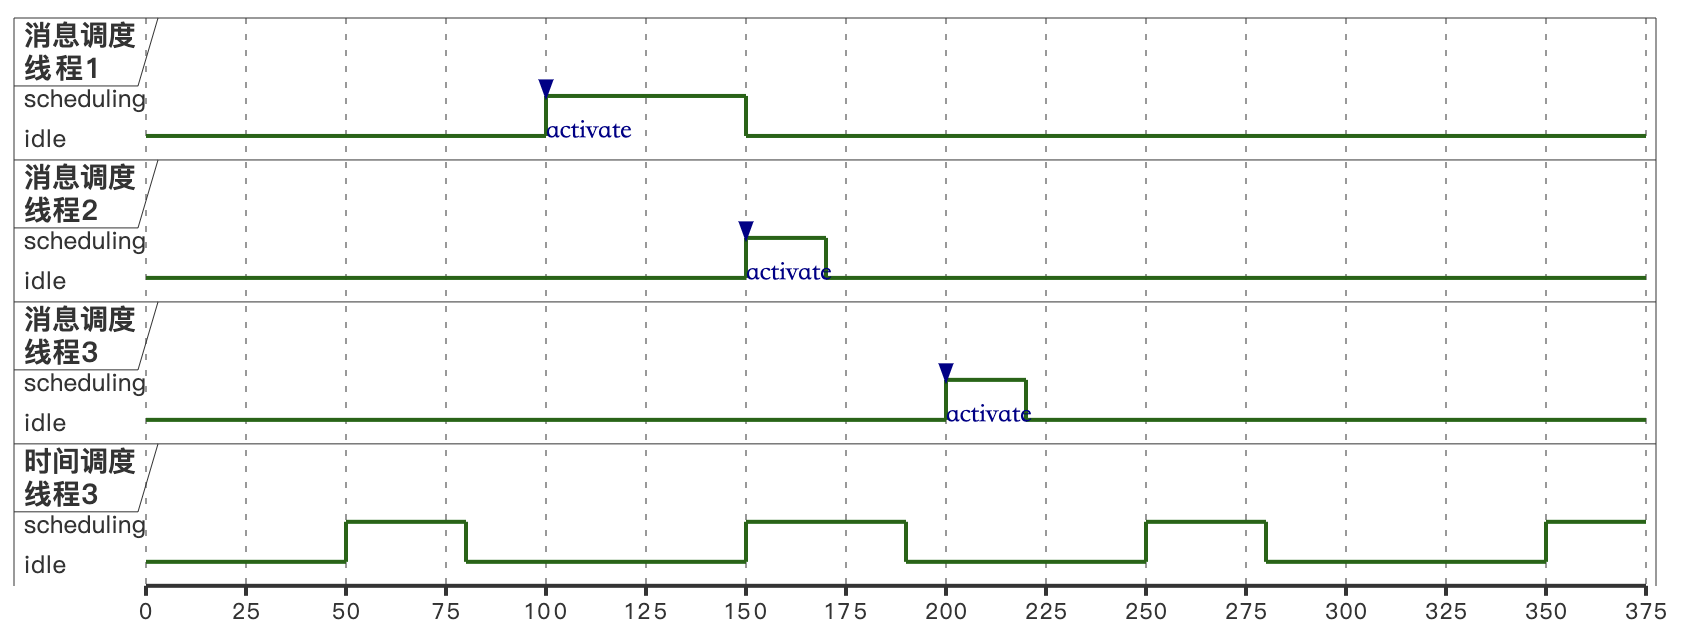
\includegraphics[width=0.95\textwidth]{5.20.png}
  \caption{任务调度模块线程运行图}
  \label{thread_running}
\end{figure}


\section{中心节点详细设计与实现}
本系统将中心节点从整个自动驾驶运行时通信系统独立出来单独实现,作为一个独立的模块开发。
中心节点提供的服务名称及其功能如表\ref{master}所示,中心节点提供的所有RPC服务全部由服务发现模块进行请求。


\begin{longtable}{lll}
  \caption{中心节点服务}\label{master}\\
  % 表格“首页”显示内容
  \toprule
  服务名称 & 服务功能 & 请求参数\\
  \midrule
  \endfirsthead
  % “后续页面”表头显示内容
  \multicolumn{2}{r}{续表\ref{master}}\\
  \toprule
  服务名称 & 服务功能 & 请求参数\\
  \hline
  %\midrule
  \endhead
  % 表格“尾页前”,表格最后显示内容
  %\bottomrule
  \endfoot
  % 表格“尾页”,表格最后显示内容
  \bottomrule
  \endlastfoot

  start\_notify & 服务发现模块向中心节点注册信息 & IP地址,端口号\\
  stop\_notify & 服务发现模块向中心节点删除信息 & IP地址,端口号\\
  create\_publisher & 创建发布者 & IP地址,发布者信息\\
  create\_subscriber & 创建订阅者 & IP地址,订阅者信息\\
  create\_service\_server & 创建服务端 & IP地址,服务端信息\\
  delete\_publisher & 删除发布者 & IP地址,发布者信息\\
  \hline
  delete\_subscriber & 删除订阅者 & IP地址,发布者信息\\
  modify\_publisher\_domain & 修改发布者通信域 & IP地址,发布者信息\\
  modify\_subscriber\_domain & 修改订阅者通信域 & IP地址,订阅者信息\\
  modify\_service\_server\_domain & 修改服务端通信域 & IP地址,服务端信息\\
  query\_publishers\_info & 查询网络内发布者信息 & 查询类型,通信域,话题名称\\
  query\_subscribers\_info & 查询网络内订阅者信息 & 查询类型,通信域,话题名称\\
  query\_service\_info & 查询网络内服务端信息 & 查询类型,通信域,服务名称\\
  lookup\_for\_service & 查询目标服务端信息 & 通信域,服务名称\\
  \end{longtable}  

% \begin{table}[H]
%   \centering\small
%   \caption{中心节点服务}
%   \label{master}
%   \begin{tabular}{lll}
%     \toprule
%     服务名称 & 服务功能 & 请求参数\\
%     \midrule
%     start\_notify & 服务发现模块向中心节点注册信息 & IP地址,端口号\\
%     stop\_notify & 服务发现模块向中心节点删除信息 & IP地址,端口号\\
%     create\_publisher & 创建发布者 & IP地址,发布者信息\\
%     create\_subscriber & 创建订阅者 & IP地址,订阅者信息\\
%     create\_service\_server & 创建服务端 & IP地址,服务端信息\\
%     delete\_publisher & 删除发布者 & IP地址,发布者信息\\
%     delete\_subscriber & 删除订阅者 & IP地址,发布者信息\\
%     modify\_publisher\_domain & 修改发布者通信域 & IP地址,发布者信息\\
%     modify\_subscriber\_domain & 修改订阅者通信域 & IP地址,订阅者信息\\
%     modify\_service\_server\_domain & 修改服务端通信域 & IP地址,服务端信息\\
%     query\_publishers\_info & 查询网络内发布者信息 & 查询类型,通信域,话题名称\\
%     query\_subscribers\_info & 查询网络内订阅者信息 & 查询类型,通信域,话题名称\\
%     query\_service\_info & 查询网络内服务端信息 & 查询类型,通信域,服务名称\\
%     lookup\_for\_service & 查询目标服务端信息 & 通信域,服务名称\\
%     \bottomrule
%   \end{tabular}
% \end{table}

中心节点除了将表\ref{master}的服务绑定至自身的RPC服务器之外,自身还实现两个重要功能:保存网络拓扑信息至本地和从本地读取网络拓扑信息。
中心节点每处理一个来自服务发现模块的RPC请求后,会将当前网络拓扑信息按照存储模型转换为json文件并保存在本地。中心节点在异常退出并被
重新运行后首先读取本地的json文件将此前的网络拓扑信息恢复。

中心节点是整个通信系统建立通信链路的关键,为了获取中心节点的运行状态本系统为中心节点开发了一个用于监控中心节点运行状态的
脚本。该脚本每隔5秒钟使用linux中的pgref -f命令查询中心节点的进程号,若查询结果为空则认为中心节点异常退出并在脚本
内重新启动中心节点程序。

\section{本章小结}
本章在第四章概要设计的基础之上,结合类图和时序图阐述了自动驾驶运行时通信系统各模块的具体实现。本章重点从通信方式自适应选择算法和
基于共享内存的进程间通信机制算法展开对本系统核心功能的描述。

